\documentclass[12pt,openany]{report}

% ==== Paquetes necesarios (Cargados una sola vez sin duplicados) ====
\usepackage{amssymb}
\usepackage{tikz}
\usepackage{afterpage}
\usepackage[most]{tcolorbox}
\usepackage{graphicx}
\newcounter{pagebeforecert}
\usepackage{xcolor}
\usepackage{fontawesome5}
\usetikzlibrary{arrows.meta,positioning,shapes.geometric,fit,calc}

\usepackage{array}
\usepackage{tabularx}
\usepackage{ragged2e} 
\usepackage{colortbl}
\usepackage{adjustbox}
\usepackage{parskip} % Esto elimina la sangría y justifica de forma limpia

\usepackage[utf8]{inputenc}
\usepackage[T1]{fontenc}
\usepackage[spanish, es-nodecimaldot]{babel}
\usepackage{helvet}
\renewcommand{\familydefault}{\sfdefault}
\usepackage{microtype}
\usepackage{longtable}
\usepackage{enumitem}
\usepackage[table,xcdraw]{xcolor}

% ======================================================================
% GEOMETRÍA GLOBAL (Márgenes exactos del SMS)
% ======================================================================
\usepackage{geometry}
\geometry{letterpaper, top=4.7cm, bottom=2.1cm, left=2.1cm, right=2.1cm, headheight=50pt, headsep=2.5cm}
\usepackage{multirow}
\usepackage{fancyhdr}
\usepackage{setspace}
\onehalfspacing

\usepackage[hidelinks]{hyperref}
\hypersetup{
  pdftitle={Manual de Control de Mantenimiento Skyfilms},
  pdfauthor={Skyfilms},
  pdfsubject={RAC 100 - Manual de Control de Mantenimiento},
  pdfcreator={LaTeX},
  pdfproducer={Overleaf}
}
\usepackage{float}
\usepackage{longtable, booktabs}
\usepackage{enumitem}
\usepackage{csquotes}
\usepackage[acronym]{glossaries}
\makeglossaries
% --- Acrónimos y abreviaturas ---

\newacronym{aaae}{AAAE}{Autoridad Aeronáutica de la Aviación de Estado}
\newacronym{aac}{AAC}{Autoridad de Aeronáutica Civil}
\newacronym{agl}{AGL}{Altura sobre el nivel del terreno}
\newacronym{arp}{ARP}{Punto de referencia del aeródromo}
\newacronym{atc}{ATC}{Servicio de control de tránsito aéreo}
\newacronym{ats}{ATS}{Servicios de tránsito aéreo}
\newacronym{bvlos}{BVLOS}{Beyond Visual Line of Sight}
\newacronym{cdm}{CDM}{Toma de decisiones en colaboración}
\newacronym{ceac}{CEAC}{Centro de entrenamiento de aeronáutica civil}
\newacronym{ciac}{CIAC}{Centro de instrucción de aeronáutica civil}
\newacronym{conops}{CONOPS}{Concepto de Operaciones}
\newacronym{dona}{DONA}{Dirección de Operaciones de Navegación Aérea}
\newacronym{evlos}{EVLOS}{Visibilidad en línea de vista extendida}
\newacronym{fato}{FATO}{Área de aproximación final y despegue}
\newacronym{fhss}{FHSS}{Frequency Hopping Spread Spectrum}
\newacronym{fpv}{FPV}{First Person View}
\newacronym{gnss}{GNSS}{Sistema Global de Navegación por Satélite}
\newacronym{metar}{METAR}{Meteorological Aerodrome Report}
\newacronym{mo}{MO}{Manual de Operaciones}
\newacronym{notam}{NOTAM}{Notice to Airmen}
\newacronym{opsp}{OpSpecs}{Especificaciones Operacionales}
\newacronym{osd}{OSD}{Telemetría en pantalla}
\newacronym{pmbo}{PMBO}{Peso máximo bruto de operación}
\newacronym{pmu}{PMU}{Puesto de mando unificado}
\newacronym{racae}{RACAE}{Reglamento Aeronáutico Colombiano de la Aviación de Estado}
\newacronym{rca}{RAC}{Reglamentos Aeronáuticos de Colombia}
\newacronym{rce}{RCE}{Responsabilidad Civil Extracontractual}
\newacronym{rpa}{RPA}{Aeronave pilotada a distancia}
\newacronym{rpas}{RPAS}{Sistema de aeronave pilotada a distancia}
\newacronym{sa}{SA}{Área de seguridad}
\newacronym{sarps}{SARPS}{Normas y métodos recomendados publicados por la OACI}
\newacronym{sms}{SMS}{Sistema de Gestión de la Seguridad Operacional}
\newacronym{taf}{TAF}{Terminal Aerodrome Forecast (Pronóstico de Aeródromo)}
\newacronym{tlof}{TLOF}{Área de contacto y elevación.}
\newacronym{ua}{UA}{Aeronave no tripulada}
\newacronym{uas}{UAS}{Sistema de Aeronaves no Tripuladas}
\newacronym{vlos}{VLOS}{Visual Line of Sight}
\newacronym{vmc}{VMC}{Condiciones meteorológicas visuales}
\newacronym{vtol}{VTOL}{Vertical Take-Off and Landing / Despegue y aterrizaje vertical}
\newacronym{znvd}{ZNVD}{Zona de No Vuelo Dron}

\usepackage[backend=biber,style=ieee]{biblatex}
\addbibresource{referencias.bib}

% ======================================================================
% AJUSTE NATIVO DEL ESPACIO EN INICIOS DE CAPÍTULO (Igual al SMS)
% ======================================================================
\makeatletter
% Modificamos la macro original de LaTeX que inserta el espacio en blanco gigante
\def\@makechapterhead#1{%
  % El valor original es \vspace*{50\p@}. Lo cambiamos a 0 o negativo para subirlo
  \vspace*{-20\p@}% <--- ESTE ES EL NÚMERO QUE PUEDES CAMBIAR (ej: -10, -30)
  {\parindent \z@ \raggedright \normalfont
    \interlinepenalty\@M
    \Huge \bfseries #1\par\nobreak
    \vskip 40\p@
  }}
\def\@makeschapterhead#1{%
  \vspace*{-20\p@}% 
  {\parindent \z@ \raggedright
    \normalfont
    \interlinepenalty\@M
    \Huge \bfseries #1\par\nobreak
    \vskip 40\p@
  }}
\makeatother
% ======================================================================

% ======================================================================
% CONFIGURACIÓN DEL ENCABEZADO INSTITUCIONAL MCM (POSICIÓN CONGELADA)
% ======================================================================
\pagestyle{fancy}
\fancyhf{}
\renewcommand{\headrulewidth}{0pt}

% Creamos una "plantilla" única para garantizar que sea 100% idéntico en toda hoja
\newcommand{\EncabezadoMCM}{%
    \renewcommand{\arraystretch}{1.6}
    \begin{tabular}{|m{3.8cm}|m{6.5cm}|m{4.8cm}|}
        \hline
        % Limitamos la altura a 2.3cm para que nunca desborde el margen superior
        \multirow{3}{3.8cm}{\centering 
\includegraphics[width=3.5cm, height=3.5cm, keepaspectratio]{Imagenes/LOGO.png}} & 
        \multirow{3}{6.5cm}{\\[0.1cm]\centering \textbf{MANUAL DE CONTROL DE}\\[0.1cm] \textbf{MANTENIMIENTO MCM}} & 
        \textbf{Versión: 1.0} \\
        \cline{3-3}
        & & \textbf{Código: MCM-SKY-001} \\
        \cline{3-3}
        & & \textbf{Fecha de Emisión: 23/06/2026} \\
        \hline
    \end{tabular}%
}

% Asignamos la plantilla a las páginas normales del desarrollo
\fancyhead[C]{\EncabezadoMCM}
\fancyfoot[R]{\thepage}

% Asignamos EXACTAMENTE la misma plantilla a los inicios de capítulo (\chapter)
\fancypagestyle{plain}{
    \fancyhf{}
    \renewcommand{\headrulewidth}{0pt}
    \fancyhead[C]{\EncabezadoMCM}
    \fancyfoot[R]{\thepage}
}
% ======================================================================

\begin{document}
\begin{titlepage}
    \centering
    {\Large \textbf{SKYFILMS}}\\[6pt]
    {\huge \textbf{Manual de Control de Mantenimiento}}\\[6pt]
    {\Large \textbf{MCM}}\\[6pt]
    {\large Cumplimiento RAC 100}\\[12pt]
    
\includegraphics[width=0.6\textwidth]{Imagenes/LOGO.png}\\[16pt]
    \begin{tabular}{ll}
    \\
    \\
    \\
    \\
    \\
    \\
    
        \textbf{Código}: & MCM-SKY-001\\
        \textbf{Versión}: & 1.0 \\
            
    \end{tabular}
    \vfill
\end{titlepage}

\chapter*{Lista de Páginas Efectivas}
\addcontentsline{toc}{chapter}{Lista de Páginas Efectivas}

La presente Lista de Páginas Efectivas (LEP) sirve como el instrumento de control documental principal para verificar la vigencia de cada una de las secciones del Manual de Control de Mantenimiento (MCM) de SKYFILMS. El Director de Mantenimiento es el responsable de mantener esta tabla actualizada con cada revisión o enmienda aprobada por la Aerocivil.

\vspace{0.3cm}
\begin{longtable}{|p{0.20\textwidth}|p{0.38\textwidth}|p{0.12\textwidth}|p{0.12\textwidth}|p{0.14\textwidth}|}
\hline
\rowcolor{gray!30}
\textbf{Cap. / Sección} & \textbf{Título de la Sección} & \textbf{Páginas} & \textbf{Revisión} & \textbf{Fecha} \\ \hline
\endhead

Preliminares & Lista de Páginas Efectivas & 1 -- 2 & 1.0 & 02/06/2026 \\ \hline
Preliminares & Control de Enmiendas y Revisiones & 3 -- 4 & 1.0 & 02/06/2026 \\ \hline
Preliminares & Lista de Distribución del Manual & 5 & 1.0 & 02/06/2026 \\ \hline
Preliminares & Definiciones y Abreviaturas & 6 -- 9 & 1.0 & 02/06/2026 \\ \hline
Preliminares & Índice General & 10 -- 12 & 1.0 & 02/06/2026 \\ \hline

Capítulo 1 & Introducción y Objetivos Generales & 13 -- 15 & 1.0 & 02/06/2026 \\ \hline
Capítulo 2 & Política y Objetivos de Mantenimiento & 16 -- 22 & 1.0 & 02/06/2026 \\ \hline
Capítulo 3 & Organización y Responsabilidades del Personal & 23 -- 32 & 1.0 & 02/06/2026 \\ \hline
Capítulo 4 & Procedimientos de Control de Mantenimiento & 33 -- 45 & 1.0 & 02/06/2026 \\ \hline
Capítulo 5 & Registros de Mantenimiento y Almacenamiento & 46 -- 52 & 1.0 & 02/06/2026 \\ \hline
Capítulo 6 & Gestión de Riesgos y Seguridad en el Taller & 53 -- 60 & 1.0 & 02/06/2026 \\ \hline
Capítulo 7 & Aseguramiento de la Calidad de Mantenimiento & 61 -- 68 & 1.0 & 02/06/2026 \\ \hline
Capítulo 8 & Control de Directivas de Aeronavegabilidad & 69 -- 74 & 1.0 & 02/06/2026 \\ \hline
Capítulo 9 & Tipos de Mantenimiento Aplicables & 75 -- 79 & 1.0 & 02/06/2026 \\ \hline
Capítulo 10 & Programa de Mantenimiento (PM) & 80 -- 84 & 1.0 & 02/06/2026 \\ \hline
Capítulo 11 & Componentes y Limitaciones de Aeronavegabilidad & 85 -- 88 & 1.0 & 02/06/2026 \\ \hline
Capítulo 12 & Capacidad Técnica e Instrucción del Personal & 89 -- 91 & 1.0 & 02/06/2026 \\ \hline

Sección Final & Anexos y Formatos Estandarizados & 92 -- 94 & 1.0 & 02/06/2026 \\ \hline
\end{longtable}
\vspace{0.3cm}

\chapter*{Control Manual Enmiendas y Revisiones}
\addcontentsline{toc}{chapter}{Control Manual Enmiendas y Revisiones}
El Manual de Control de Mantenimiento (MCM) de \textbf{SKYFILMS} está sujeto a un control documental estricto. Cualquier cambio relacionado con la normativa, modificación, incorporación o eliminación en el contenido deberá registrarse mediante un proceso formal, con el objetivo de garantizar la coherencia técnica, la trazabilidad de los cambios y el estricto cumplimiento de los Reglamentos Aeronáuticos de Colombia (RAC 100 y RAC 219).

Para asegurar un correcto seguimiento, \textbf{SKYFILMS} clasifica las modificaciones del manual en dos categorías:

\begin{itemize}
    \item \textbf{Revisiones:} Corresponden a cambios menores, correcciones de redacción, actualizaciones de datos específicos o sustitución de páginas individuales que no alteran la estructura general del documento.

    \item \textbf{Enmiendas (Versiones):} Corresponden a cambios estructurales mayores, incorporaciones de nuevas normativas, cambios en la flota UAS o reemisiones completas del documento que ameritan un cambio en el número de versión oficial.
\end{itemize}

Toda revisión o enmienda será documentada en sus respectivos formatos de control y quedará reflejada en las secciones pertinentes. La versión oficial y vigente será almacenada como copia maestra en el sistema digital centralizado de \textbf{SKYFILMS}, garantizando que las copias obsoletas distribuidas al personal sean retiradas y sustituidas en cada actualización.\\

\textbf{1. REGISTRO DE REVISIONES}

Las revisiones se realizan para mantener el manual actualizado de manera ágil ante cambios operativos puntuales. Cada revisión menor incluirá un registro detallado para conocer exactamente qué parte del documento fue intervenida.

A continuación, se presenta la tabla de control, cuyo contenido se diligenciará de la siguiente manera:

\begin{itemize}
    \item \textbf{Revisión:} Número secuencial asignado al cambio menor.

    \item \textbf{Página:} Número exacto de la página (o páginas) donde se refleja el ajuste.

    \item \textbf{Fecha de Aplicación:} Fecha a partir de la cual la directriz, norma o cambio operativo entra en vigor en las operaciones de \textbf{SKYFILMS}.

    \item \textbf{Fecha de Inserción:} Fecha real en la que el documento maestro fue editado y actualizado en el sistema.

    \item \textbf{Insertado por:} Nombre y cargo de la persona encargada de realizar la modificación física o digital en el documento.
\end{itemize}

\begin{table}[H]
\begin{adjustbox}{center}
\renewcommand{\arraystretch}{1.5} % Controla la altura de las filas para que se vean espaciosas
\begin{tabular}{|>{\centering\arraybackslash}m{0.12\linewidth}|>{\centering\arraybackslash}m{0.12\linewidth}|>{\centering\arraybackslash}m{0.22\linewidth}|>{\centering\arraybackslash}m{0.22\linewidth}|>{\centering\arraybackslash}m{0.22\linewidth}|}
\hline
% Puedes cambiar 'gray!20' por tu color de encabezado si ya tienes uno definido (ej. headerblue)
\rowcolor{gray!20} 
\textbf{Revisión} & \textbf{Página} & \textbf{Fecha de Aplicación} & \textbf{Fecha de Inserción} & \textbf{Insertado por} \\
\hline
 & & & & \\ \hline
 & & & & \\ \hline
 & & & & \\ \hline
 & & & & \\ \hline
\end{tabular}
\end{adjustbox}
\caption{Registro de Revisiones}
\label{tab:registro_revisiones}
\end{table}

\textbf{2. REGISTRO DE ENMIENDAS (CONTROL DE VERSIONES)}

Las enmiendas representan evoluciones significativas en el MCM de la organización. A diferencia de las revisiones, una enmienda requiere una descripción clara del contexto del cambio y la validación formal de la alta gerencia, ya que impacta la integridad general del manual.

A continuación, se presenta la tabla de control de versiones, cuyo contenido se diligenciará de la siguiente manera:

\begin{itemize}
    \item \textbf{Versión:} Número oficial del manual tras la enmienda mayor.

    \item \textbf{Página:} Identificación de los capítulos, anexos o el total de páginas que fueron reestructurados.

    \item \textbf{Fecha:} Fecha oficial de emisión, aprobación y publicación de la nueva versión del manual.

    \item \textbf{Descripción Resumida del Cambio:} Explicación breve y precisa del motivo de la enmienda (Ej. Actualización integral por entrada en vigencia de la Directiva \#\#-\#\# de Aerocivil).

    \item \textbf{Responsable:} Nombre de la autoridad aeronáutica interna que valida y aprueba la emisión de la nueva versión.
\end{itemize}

\begin{table}[H]
\begin{adjustbox}{center}
\renewcommand{\arraystretch}{1.5} % Controla la altura de las filas para que se vean espaciosas
\begin{tabular}{|>{\centering\arraybackslash}m{0.12\linewidth}|>{\centering\arraybackslash}m{0.12\linewidth}|>{\centering\arraybackslash}m{0.15\linewidth}|>{\centering\arraybackslash}m{0.32\linewidth}|>{\centering\arraybackslash}m{0.2\linewidth}|}
\hline
% Puedes cambiar 'gray!20' por tu color de encabezado si ya tienes uno definido (ej. headerblue)
\rowcolor{gray!20} 
\textbf{Versión} & \textbf{Página} & \textbf{Fecha} & \textbf{Descripción Resumida del Cambio} & \textbf{Responsable} \\
\hline
 & & & & \\ \hline
 & & & & \\ \hline
 & & & & \\ \hline
 & & & & \\ \hline
\end{tabular}
\end{adjustbox}
\caption{Registro de Versiones}
\label{tab:registro_enmiendas}
\end{table}

\chapter*{Lista de Distribución}
\addcontentsline{toc}{chapter}{Lista de Distribución}
La distribución del Manual sigue el procedimiento del Manual de Operaciones: el Gerente General autoriza, el Gerente SMS entrega la copia dentro de los cinco (5) días hábiles siguientes y cada receptor firma el acuse de recibo (F-015).

\begin{longtable}{|p{6cm}|p{3cm}|p{4.5cm}|}
\hline
\rowcolor{gray!30}
\textbf{Rol} & \textbf{Formato} & \textbf{Responsable de la entrega} \\ \hline
\endhead
Gerente General & PDF (editable) & Gerente SMS \\ \hline
Gerente de Seguridad Operacional (Gerente SMS) & PDF (editable) & Gerente SMS \\ \hline
Jefe de Pilotos UAS & PDF & Gerente SMS \\ \hline
Técnico UAS (Responsable de Mantenimiento) & PDF (editable) & Gerente SMS \\ \hline
Pilotos remotos y observadores visuales (consulta de los capítulos que les aplican) & PDF & Gerente SMS \\ \hline
Aerocivil (versión aprobada y enmiendas sustanciales) & PDF & Gerente General \\ \hline
\end{longtable}


\chapter*{Declaración de Cumplimiento}
\addcontentsline{toc}{chapter}{Declaracion de Cumplimiento}
En cumplimiento de lo dispuesto en el Decreto 1294 de 2021, el Convenio de Chicago de 1944 y el Reglamento Aeronáutico Colombiano RAC 100, Skyfilms, como explotador de Sistemas de Aeronaves No Tripuladas (UAS), en la Categoría Específica para operaciones de simple captura de imágenes o datos, emite la presente Declaración de Cumplimiento:

\begin{enumerate}
    \item Skyfilms manifiesta que todas sus operaciones con UAS se desarrollan en estricto apego a las disposiciones establecidas en el RAC 100 y demás normas aeronáuticas vigentes en la República de Colombia.
    \item La empresa se compromete a implementar los procedimientos descritos en el Manual de Operaciones y SMS, asegurando la gestión de riesgos, la protección de terceros y la preservación de la seguridad operacional en todas sus actividades.
    \item Se reconoce la autoridad de la Unidad Administrativa Especial de Aeronáutica Civil como ente regulador, certificador y supervisor de las operaciones aéreas con UAS en el territorio nacional.
    \item Skyfilms se obliga a mantener actualizada la información contenida en este Manual, introduciendo las modificaciones necesarias cuando existan cambios normativos, técnicos u operacionales, y a someter dichas modificaciones a la aprobación de la Aerocivil.
    \item Todo el personal vinculado a Skyfilms S.A.S. está en obligación de conocer y aplicar estrictamente todos los procesos y procedimientos en este manual.
\end{enumerate}

\vspace{1cm}

\begin{center}


\includegraphics[width=4cm]{Imagenes/firma.jpg}

\vspace{-1.2cm}

\rule{7cm}{0.5pt}

\vspace{0.3cm}
\textbf{Andrés Felipe Pérez Sierra}\\
C.C. 1.108.206.142\\
Gerente General\\


\end{center}

\tableofcontents
\clearpage

% Capítulo 1: Información General
\chapter{Introducción}
\label{chap:introduccion}

El presente Manual de Control de Mantenimiento (MCM) de SKYFILMS ha sido elaborado con el propósito de establecer las políticas, procedimientos, responsabilidades y estándares que rigen la gestión del mantenimiento de los Sistemas de Aeronaves No Tripuladas (UAS) operados por la organización.\\

Este manual constituye el documento oficial de referencia técnica y administrativa para asegurar que todas las actividades de mantenimiento preventivo, correctivo, de inspección y control técnico de los equipos se realicen conforme a los Reglamentos Aeronáuticos de Colombia (RAC 100) y a las directrices emitidas por la Unidad Administrativa Especial de Aeronáutica Civil (Aerocivil).\\

El MCM busca garantizar que la flota de UAS de SKYFILMS se mantenga en condiciones de aeronavegabilidad continuada, preservando en todo momento la seguridad operacional, la confiabilidad técnica y la eficiencia de las operaciones aéreas realizadas con fines de producción audiovisual, fotografía aérea y servicios relacionados.\\

Asimismo, este documento establece los mecanismos de control documental, trazabilidad y verificación técnica, aplicables tanto al mantenimiento ejecutado directamente por SKYFILMS como al realizado por proveedores externos aceptados, bajo los lineamientos de calidad y seguridad definidos por la organización.\\

\section{Alcance}

El presente Manual aplica a todas las actividades de mantenimiento, inspección, reparación, reemplazo, control técnico y registro de los UAS pertenecientes a SKYFILMS, incluyendo sus componentes, baterías, equipos de control remoto, sensores y accesorios asociados.\\

Su alcance comprende:

\begin{itemize}
    \item Los procesos internos de mantenimiento realizados en las instalaciones de SKYFILMS.

    \item El mantenimiento tercerizado, efectuado por organizaciones o técnicos externos previamente evaluados y aceptados.

    \item Las acciones de control, documentación y seguimiento a las condiciones técnicas y de aeronavegabilidad de los UAS, durante todas las fases operacionales.

    \item La implementación de programas de mantenimiento preventivo, inspecciones periódicas, control de herramientas, manejo de baterías, almacenamiento y disposición final de componentes.
\end{itemize}

El MCM aplica al personal técnico, operativo y administrativo que participa directa o indirectamente en los procesos de mantenimiento de UAS, y es de cumplimiento obligatorio para todos los colaboradores y contratistas que realicen actividades bajo el certificado de operación de SKYFILMS.

\section{Marco Normativo y Referencias}
Este Manual se fundamenta en la normatividad aeronáutica vigente en la República de Colombia, particularmente en:

\begin{itemize}
    \item \textbf{RAC 100} – Operación de Sistemas de Aeronaves No Tripuladas (UAS).

    \item \textbf{MAUT-5.0-22-011} – Guía para obtener el certificado de explotador UAS.

    \item \textbf{MAUT-5.0-12-097FO} – Lista de verificación para revisar el Manual de Control de Mantenimiento.

    \item Manual del fabricante de cada modelo de UAS operado por SKYFILMS.
\end{itemize}

El cumplimiento de este marco normativo es obligatorio y verificable ante la Aerocivil, y todo el personal técnico de SKYFILMS deberá conocer, aplicar y mantener actualizada la información contenida en el presente documento.



% =========================================================================
% CONTROL DE MÁRGENES ESTÁNDAR POR CAPÍTULO (Igual al SMS)
% =========================================================================



% Capítulo 2: Definiciones y Abreviaturas
\newgeometry{top=4.2cm, bottom=2.5cm, left=2cm, right=2cm, headheight=50pt, headsep=2.0cm}
\chapter{Definiciones y Abreviaturas}
\label{chap:Definiciones y Abreviaturas}
El presente capítulo establece el vocabulario técnico, las definiciones regulatorias y los acrónimos utilizados en el Manual de Control de Mantenimiento (MCM) de SKYFILMS. Su objetivo es garantizar una interpretación estandarizada, precisa y libre de ambigüedades por parte de todo el personal de mantenimiento, operaciones y los inspectores de la Autoridad Aeronáutica, en conformidad con los Reglamentos Aeronáuticos de Colombia (RAC).

\section*{Abreviaturas y Acrónimos}

\begin{longtable}{|p{0.18\textwidth}|p{0.76\textwidth}|}
\hline
\rowcolor{gray!30}
\textbf{Acrónimo} & \textbf{Significado Oficial} \\ \hline
\endhead

\textbf{AOC / CDO} & Certificado de Operador Aéreo / Certificado de Explotador de Drones. \\ \hline
\textbf{ATA} & \textit{Air Transport Association} (código de capítulos para clasificar sistemas). \\ \hline
\textbf{BITE} & \textit{Built-In Test Equipment} (Equipo de Prueba Integrado o Autodiagnóstico). \\ \hline
\textbf{C2} & \textit{Command and Control Link} (Enlace de Mando y Control). \\ \hline
\textbf{COTS} & \textit{Commercial Off-The-Shelf} (Componentes comerciales de estantería o uso civil). \\ \hline
\textbf{DIACC} & Dirección de Investigación de Accidentes (de la Aerocivil). \\ \hline
\textbf{DJI} & Fabricante del Mavic 4 Pro y del sistema O4 Pro. \\ \hline
\textbf{ELRS} & \textit{ExpressLRS} (sistema de radiocontrol de largo alcance). \\ \hline
\textbf{EPP} & Elementos de Protección Personal. \\ \hline
\textbf{ESC} & \textit{Electronic Speed Controller} (Controlador Electrónico de Velocidad). \\ \hline
\textbf{ESD} & \textit{Electrostatic Discharge} (descarga electrostática). \\ \hline
\textbf{FC} & \textit{Flight Controller} (Controlador de Vuelo / Aviónica). \\ \hline
\textbf{FOD} & \textit{Foreign Object Debris} (Daño o residuo por Objetos Extraños). \\ \hline
\textbf{FPV} & \textit{First Person View} (vista en primera persona). \\ \hline
\textbf{GCS} & \textit{Ground Control Station} (Estación de Control en Tierra). \\ \hline
\textbf{GNSS} & \textit{Global Navigation Satellite System} (navegación por satélite). \\ \hline
\textbf{GPS} & \textit{Global Positioning System} (sistema de posicionamiento global). \\ \hline
\textbf{IMU} & \textit{Inertial Measurement Unit} (Unidad de Medida Inercial). \\ \hline
\textbf{LED} & \textit{Light Emitting Diode} (diodo emisor de luz). \\ \hline
\textbf{LiPo / Li-ion} & Baterías de polímero de litio / de ion de litio. \\ \hline
\textbf{LLP} & \textit{Life Limited Parts} (Partes o componentes de Vida Límite). \\ \hline
\textbf{LQ} & \textit{Link Quality} (calidad del enlace de control). \\ \hline
\textbf{MCM} & Manual de Control de Mantenimiento. \\ \hline
\textbf{MO} & Manual de Operaciones. \\ \hline
\textbf{OEM} & \textit{Original Equipment Manufacturer} (Fabricante de Equipo Original). \\ \hline
\textbf{OSD} & \textit{On-Screen Display} (datos en pantalla). \\ \hline
\textbf{P/N} & \textit{Part Number} (número de parte). \\ \hline
\textbf{PIC} & \textit{Pilot In Command} (Piloto al Mando / Piloto UAS). \\ \hline
\textbf{PM} & Programa de Mantenimiento. \\ \hline
\textbf{PRE} & Plan de Respuesta ante Emergencias. \\ \hline
\textbf{RAC} & Reglamentos Aeronáuticos de Colombia. \\ \hline
\textbf{RAEE} & Residuos de Aparatos Eléctricos y Electrónicos. \\ \hline
\textbf{RPAS / UAS} & \textit{Remotely Piloted Aircraft System / Unmanned Aircraft System} (Sistema de Aeronave No Tripulada). \\ \hline
\textbf{RSSI} & \textit{Received Signal Strength Indicator} (intensidad de la señal recibida). \\ \hline
\textbf{RTH} & \textit{Return To Home} (regreso al punto de partida). \\ \hline
\textbf{RUAS} & Registro de Unidades de Aeronaves no Tripuladas (de la Aerocivil). \\ \hline
\textbf{SB} & \textit{Service Bulletin} (boletín de servicio). \\ \hline
\textbf{SMS} & \textit{Safety Management System} (Sistema de Gestión de Seguridad Operacional). \\ \hline
\textbf{SST} & Seguridad y Salud en el Trabajo. \\ \hline
\textbf{TAT} & \textit{Turn Around Time} (tiempo de entrega de un trabajo). \\ \hline
\textbf{VLOS} & \textit{Visual Line of Sight} (línea de vista visual). \\ \hline
\textbf{VTX} & \textit{Video Transmitter} (Transmisor de Video). \\ \hline
\textbf{XBand} & Receptor ExpressLRS de banda dual instalado en el Pavo20. \\ \hline
\end{longtable}


\section*{Definiciones Técnicas y Regulatorias}

\begin{itemize}
    \item \textbf{Aeronavegabilidad:} Condición técnica, física y legal en la cual una aeronave o componente se ajusta a su diseño certificado y se encuentra en un estado operativo completamente seguro para el vuelo.
    
    \item \textbf{Aeronavegabilidad Continuada:} Conjunto de procesos, inspecciones y tareas de mantenimiento ejecutadas sistemáticamente para garantizar que el Sistema de Aeronave No Tripulada (UAS) se mantenga en condiciones seguras durante toda su vida útil.
    
    \item \textbf{Boletín de Servicio (SB - Service Bulletin):} Documento emitido por el fabricante de la aeronave o de un componente (OEM) que detalla modificaciones, inspecciones o actualizaciones de software recomendadas u obligatorias para mantener la seguridad operacional.
    
    \item \textbf{Componente de Vida Límite (LLP):} Parte crítica de la aeronave, como las hélices, baterías o motores, que debe ser retirada permanentemente del servicio tras alcanzar un parámetro preestablecido (horas de vuelo, ciclos de carga o meses calendario), sin importar su estado físico aparente.
    
    \item \textbf{Hard Time (Tiempo Límite Mandatorio):} Filosofía de mantenimiento preventivo bajo la cual un componente es removido de la aeronave de manera obligatoria al cumplirse un intervalo de tiempo específico (horas, días o ciclos) dictado en el Programa de Mantenimiento.
    
    \item \textbf{Liberación de Mantenimiento (Retorno al Servicio):} Certificación técnica registrada en el Libro de Mantenimiento y firmada por el personal autorizado de SKYFILMS, indicando que el trabajo correctivo o preventivo se ha realizado satisfactoriamente y la aeronave es apta para volar.
    
    \item \textbf{Mantenimiento Correctivo:} Acción no programada que se efectúa en un UAS o en sus equipos de soporte para aislar y reparar una falla técnica o daño estructural, restableciendo sus condiciones normales de operación.
    
    \item \textbf{Mantenimiento Mayor:} Intervención de alta complejidad que implica desensambles profundos, soldadura de componentes electrónicos, modificaciones estructurales en chasis de fibra de carbono o calibraciones profundas de sistemas que exigen herramientas metrológicas.
    
    \item \textbf{Mantenimiento Menor:} Tareas preventivas y de baja complejidad ejecutadas en la línea de vuelo, tales como inspección visual, limpieza de motores, actualización cruzada de firmware y reemplazo de partes de rápida instalación (plug-and-play).
    
    \item \textbf{Monitoring Condition (Condición Monitoreada):} Filosofía de control y mantenimiento que evalúa la salud de los subsistemas a través del análisis de datos continuos, telemetría, \textit{logs} de vuelo y alertas de los equipos de prueba integrados (BITE).
    
    \item \textbf{On Condition (A Condición):} Filosofía de mantenimiento aplicada a componentes que permanecen instalados en la aeronave hasta que una inspección física y funcional demuestre que han superado sus tolerancias de desgaste, momento en el cual son reemplazados.
    
    \item \textbf{Overhaul (Reacondicionamiento General):} Proceso técnico mayor que consiste en el desmontaje total, limpieza, inspección rigurosa, reparación y prueba funcional de motores u otros ensambles, restituyéndolos a sus tolerancias originales de fábrica.
\end{itemize}

% Capítulo 3: Estructura organizacional y responsabilidades
\newgeometry{top=4.2cm, bottom=2.5cm, left=2cm, right=2cm, headheight=50pt, headsep=2.0cm}
\chapter{Estructura Organizacional y Responsabilidades}
\label{chap:Estructura organizacional y responsabilidades}
La estructura organizacional del área de mantenimiento de SKYFILMS se ha diseñado para asegurar un flujo jerárquico claro cumplimiento de los requisitos establecidos por la Unidad Administrativa Especial de Aeronáutica Civil (Aerocivil) para explotadores de Sistemas de Aeronaves No Tripuladas (UAS), conforme al RAC 100.\\

El objetivo de esta estructura es garantizar que las decisiones técnicas relacionadas con el mantenimiento y la aeronavegabilidad continuada sean adoptadas por personal competente y autorizado, evitando conflictos de interés entre las áreas operativas y de control técnico.
La estructura organizacional también define con precisión las funciones, responsabilidades y autoridad de cada cargo vinculado al proceso de mantenimiento.

\section{Estructura Organizacional}
El área técnica de SKYFILMS está compuesta por los siguientes niveles jerárquicos:

\subsection{Descripción general de la estructura}
El área de mantenimiento de SKYFILMS está compuesta por los siguientes niveles jerárquicos y de responsabilidad:

\begin{itemize}

    \item \textbf{Gerente General}
    \item \textbf{Técnico UAS} (corresponde al Responsable de Mantenimiento del Manual de Operaciones)

\end{itemize}

Estos cargos conforman la estructura técnica mínima requerida para garantizar la operación segura y la gestión efectiva del mantenimiento. El Jefe de Pilotos UAS y el Gerente SMS (SMS) (en adelante, Gerente SMS) apoyan el proceso desde sus propias funciones, como se describe a continuación, y no forman parte de la cadena de liberación de aeronaves.

\subsection{Perfil y competencias del Técnico UAS}
\begin{itemize}
    \item Formación técnica o experiencia demostrable en aeronaves no tripuladas, electrónica o mecánica, verificada por el Gerente General antes de su designación. Su autorización inicial y sus límites están en el capítulo de capacidad técnica del personal.
    \item Entrenamiento inicial y recurrente según el capítulo de capacidad técnica del personal, y entrenamiento específico en el Mavic 4 Pro y en el Pavo20 Pro II.
    \item Conocimiento del RAC 100, del Manual de Operaciones, del SMS y de este Manual.
    \item Es la única persona autorizada para liberar una aeronave al servicio. Si no está disponible, no se libera ninguna aeronave y el mantenimiento se realiza con un proveedor aceptado (capítulo de proveedores). El Gerente General puede designar por escrito un reemplazo temporal que cumpla este perfil.
\end{itemize}

\subsection{Representación gráfica}
La estructura jerárquica y funcional se representa de la siguiente manera:

\begin{figure}[H]
\centering
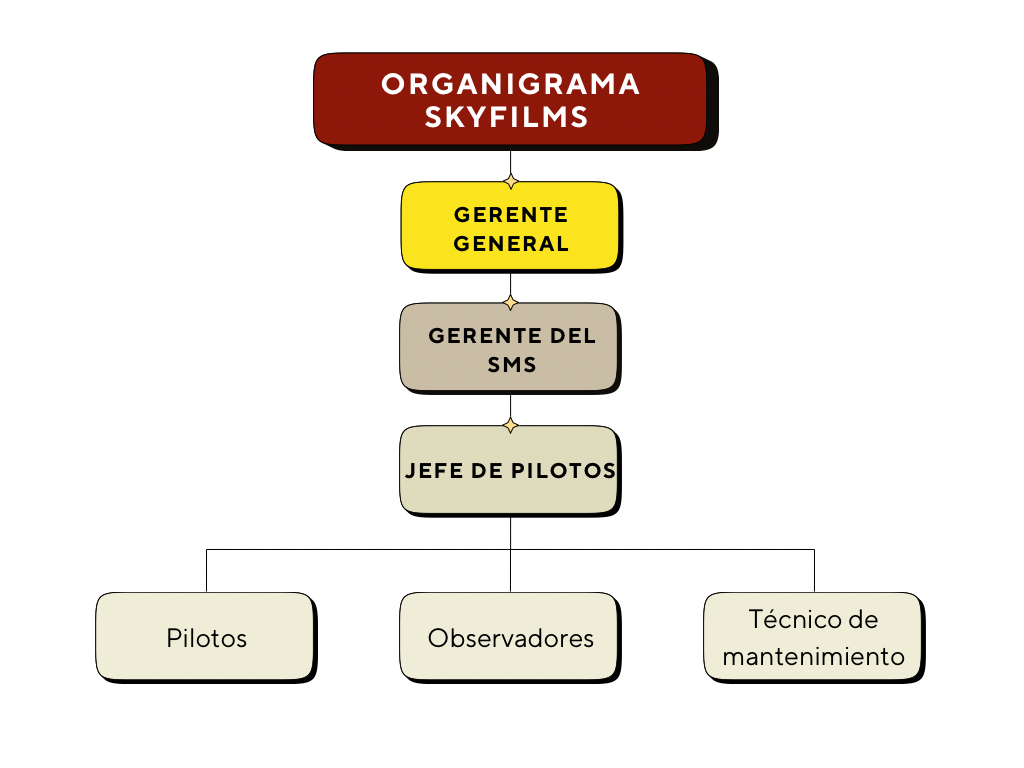
\includegraphics[width=.85\textwidth]{Imagenes/organigrama_skyfilm.PNG}
\caption{Estructura MCM Skyfilms}
\end{figure}


Esta representación refleja las líneas de autoridad, coordinación e intercambio de información entre las áreas de mantenimiento, seguridad operacional y operaciones de vuelo.

\section{Funciones y Responsabilidades del Personal}

\begin{enumerate}
    \item \textbf{Gerente General}
        \begin{itemize}
            \item Garantizar que la organización cumpla con las disposiciones del RAC 100 y con las políticas definidas por la Aerocivil.
            \item Aprobar el Manual de Control de Mantenimiento y sus revisiones.
            \item Asignar los recursos humanos, financieros y técnicos necesarios para el cumplimiento del Programa de Mantenimiento.
            \item Asegurar la coordinación efectiva entre las áreas de Mantenimiento, Operaciones y Seguridad Operacional.
            \item Mantener comunicación directa con la Aerocivil respecto a los temas de mantenimiento, enmiendas al MCM y cumplimiento regulatorio.
            \item Actuar como directivo responsable: responde ante la Aerocivil por que Skyfilms cumpla lo que dice este Manual y por que existan los recursos para ejecutarlo.
        \end{itemize}
    \item \textbf{Tecnico UAS}
        \begin{itemize}
            \item \textbf{Ejecución técnica:} Realizar inspecciones, mantenimientos, pruebas funcionales y calibraciones según los programas aprobados, asegurando la aeronavegabilidad de los UAS.

            \item \textbf{Registro y trazabilidad:} Diligenciar correctamente los formatos de mantenimiento, libros técnicos y reportes de servicio, garantizando la veracidad y oportunidad de la información registrada.

            \item \textbf{Uso adecuado de herramientas:} Emplear únicamente equipos, instrumentos y materiales certificados y en condiciones óptimas.

            \item \textbf{Cumplimiento normativo:} Aplicar los procedimientos, políticas de seguridad operacional y estándares técnicos establecidos por SKYFILMS y la Aerocivil.

            \item \textbf{Gestión de seguridad:} Reportar de manera inmediata cualquier hallazgo, daño o condición insegura que afecte la operación o el mantenimiento.

            \item \textbf{Apoyo en la gestión técnica:} Colaborar en la actualización del inventario de herramientas, componentes y registros técnicos bajo supervisión del Jefe de Pilotos y del Gerente General.

            \item \textbf{Control documental:} Asegurar que todos los documentos utilizados correspondan a versiones vigentes y que los registros se archiven conforme al sistema de gestión documental del MCM.

            \item \textbf{Factores humanos:} Mantener condiciones físicas y mentales adecuadas para el desempeño de sus labores, evitando trabajar bajo fatiga, estrés o presión excesiva.
        \end{itemize}
    \item \textbf{Gerente SMS}
        \begin{itemize}
            \item Velar porque las actividades de mantenimiento estén integradas al Sistema de Gestión de Seguridad Operacional (SMS).
            \item Analizar riesgos derivados del mantenimiento, proponiendo medidas de mitigación.
            \item Revisar reportes de eventos o incidentes relacionados con mantenimiento y emitir alertas de seguridad.
            \item Promover la cultura de seguridad y la gestión de factores humanos en el área técnica.
            \item Coordinar con el Técnico UAS (Responsable de Mantenimiento) la implementación de acciones correctivas y preventivas.
            \item Controlar la calidad y el riesgo del trabajo técnico: revisa por muestreo los registros de mantenimiento y verifica que se cumplan las listas de chequeo, sin firmar la liberación de aeronaves.
        \end{itemize}
    \item \textbf{Jefe de Pilotos UAS}
        \begin{itemize}
            \item Mantener comunicación constante con el área técnica para informar cualquier condición anómala detectada en operación.
            \item Colaborar con el Tecnico UAS en la realización de pruebas funcionales posteriores al mantenimiento.
            \item Garantizar que los pilotos registren correctamente las discrepancias técnicas en los formatos establecidos.
            \item Supervisar que la operación de vuelo se realice únicamente con aeronaves que posean condición aeronavegable certificada.
        \end{itemize}

\end{enumerate}

\textbf{Representante del proveedor externo:} cuando exista una organización de mantenimiento aceptada, su representante técnico firma los informes de los trabajos y responde por ellos ante Skyfilms (ver el capítulo de proveedores).

\section{Responsabilidad y Cumplimiento}
Todos los miembros del área técnica son responsables de:

\begin{itemize}
    \item Cumplir estrictamente las disposiciones contenidas en el presente Manual de Control de Mantenimiento y en las regulaciones RAC.
    \item Contribuir al mantenimiento de la aeronavegabilidad continuada y a la seguridad operacional de las operaciones UAS de SKYFILMS.
    \item Notificar de manera inmediata cualquier desviación, no conformidad o situación que afecte la seguridad o el cumplimiento normativo.
\end{itemize}

El Gerente General y el Tecnico UAS asumen la responsabilidad final ante la Aerocivil por el cumplimiento del presente manual y la integridad técnica de la flota UAS de SKYFILMS.

% Capítulo 4: Descripción de las aeronaves UAS
\newgeometry{top=4.2cm, bottom=2.5cm, left=2cm, right=2cm, headheight=50pt, headsep=2.0cm}
\chapter{Descripción de las aeronaves UAS}
\label{chap:Descripción de las aeronaves UAS}
El presente capítulo tiene como finalidad identificar y describir las aeronaves no tripuladas (UAS) incluidas dentro del Certificado de Explotador UAS de SKYFILMS, así como sus principales características técnicas y operativas.\\

\textbf{NOTA:} Toda aeronave listada en este capítulo ha sido evaluada y aceptada por el Técnico UAS, quien certifica que cumple con las condiciones técnicas y documentales necesarias para ser operada dentro de las actividades autorizadas a SKYFILMS. La trazabilidad del mantenimiento de cada UA esta en el \textbf{Anexo 1 - Hoja de Vida UA}.

\begin{center}
\subsection*{DJI Mavic 4 Pro}
\begin{tabular}{|p{6cm}|p{8cm}|}
\hline
\textbf{Parámetro} & \textbf{Especificación} \\ \hline
Marca / Modelo & DJI Mavic 4 Pro \\ \hline
Número de Serie & [Por registrar] \\ \hline
Registro RUAS & [Por asignar Aerocivil] \\ \hline
Clasificación & Multirrotor VTOL \\ \hline
MTOW & 1.6 kg (ejemplo, ajustar) \\ \hline
Dimensiones físicas & 347 × 283 × 107 mm (plegado) \\ \hline
Tipo de despegue / aterrizaje & Vertical automático/manual \\ \hline
Velocidad máx. ascenso & 8 m/s \\ \hline
Velocidad máx. descenso & 6 m/s \\ \hline
Velocidad máx. vuelo & 21 m/s (75 km/h) \\ \hline
Techo máx. operación & 6000 m sobre el nivel del mar \\ \hline
Autonomía & 34–40 min (según batería y condiciones) \\ \hline
Alcance máx. & 20 km  \\ \hline
Viento máx. resistido & 12 m/s \\ \hline
Rango temperatura & –10 °C a 40 °C \\ \hline
GNSS soportados & GPS + Galileo + BeiDou + GLONASS \\ \hline
Protección IP & No aplica \\ \hline
Frecuencias Enlace C2 & 2.4 GHz, 5.1 GHz, 5.8 GHz \\ \hline
Potencia Tx & Ver especificaciones FCC/CE (hasta 33 dBm) \\ \hline
Latencia enlace C2 & 120–130 ms \\ \hline
Encriptación enlace C2 & AES 256-bit \\ \hline
Sistemas de detección & Omnidireccional, APAS 5.0 \\ \hline
Carga útil & Cámara integrada 4/3 CMOS Hasselblad \\ \hline
Estación en tierra & DJI RC Pro / DJI RC-N2 \\ \hline
\end{tabular}


\subsection*{FPV 5" 6S}
\begin{tabular}{|p{6cm}|p{8cm}|}
\hline
\textbf{Parámetro} & \textbf{Especificación} \\ \hline
Marca / Modelo & [Por definir] \\ \hline
Número de Serie & [Por registrar] \\ \hline
Registro RUAS & [Por asignar Aerocivil] \\ \hline
Clasificación & Multirrotor FPV VTOL \\ \hline
MTOW & 900 gr \\ \hline
Dimensiones físicas &  (L×W×H): 230*207*54mm \\ \hline
Tipo de despegue / aterrizaje & Vertical manual (pilotaje FPV) \\ \hline
Velocidad máx. ascenso & ~15 m/s (dependiendo configuración) \\ \hline
Velocidad máx. descenso & ~10 m/s \\ \hline
Velocidad máx. vuelo & > 160 km/h (modo acro) \\ \hline
Techo máx. operación & 5000 m (limitado por densidad de aire y motores) \\ \hline
Autonomía & 5–8 min (dependiendo batería y perfil de vuelo) \\ \hline
Alcance máx. & 5–10 km (con ELRS, condiciones ideales) \\ \hline
Viento máx. resistido & 10–12 m/s \\ \hline
Rango temperatura & –10 °C a 40 °C (operación estándar) \\ \hline
GNSS soportados & GPS+SBAS+Galileo+QZSS+Glonass \\ \hline
Protección IP & No aplica \\ \hline
Frecuencias Enlace C2 & 2.4 GHz / 915 MHz (ELRS Crossband) \\ \hline
Potencia Tx & Hasta 1 W por banda \\ \hline
Latencia enlace C2 & < 20 ms  \\ \hline
Encriptación enlace C2 & Soportada por protocolo ELRS (LoRa) \\ \hline
Sistemas de detección & No dispone de sensores de evitación \\ \hline
Carga útil & GoPro / cámaras de acción (máx. 150 g) \\ \hline
Estación en tierra & RadioMaster TX16S + Módulo ELRS Nomad \\ \hline
\end{tabular}


\end{center}

% Capítulo 5: Instalaciones
\newgeometry{top=4.2cm, bottom=2.5cm, left=2cm, right=2cm, headheight=50pt, headsep=2.0cm}
\chapter{Instalaciones}
\label{chap:Instalaciones}

Las instalaciones de SKYFILMS destinadas a las actividades de mantenimiento, inspección, almacenamiento y control técnico de los Sistemas de Aeronaves No Tripuladas (UAS) están adecuadamente equipadas y organizadas para garantizar el cumplimiento de los procedimientos establecidos en este Manual de Control de Mantenimiento (MCM) y en los Reglamentos Aeronáuticos de Colombia (RAC 100).

Estas instalaciones permiten ejecutar de manera segura y eficiente las tareas de mantenimiento preventivo, correctivo, limpieza, calibración de equipos, carga de baterías y almacenamiento de componentes, asegurando condiciones que preservan la integridad técnica de las aeronaves y la seguridad del personal.

\section{Características}
Las labores de mantenimiento se realizan en las instalaciones principales de SKYFILMS, ubicadas en Ibagué, Tolima, las cuales cuentan con un área delimitada y señalizada para la manipulación y mantenimiento de aeronaves no tripuladas.

Las áreas están organizadas de acuerdo con su función y cuentan con los elementos mínimos requeridos por la Aerocivil, incluyendo:

\begin{itemize}
    \item \textbf{Área de mantenimiento técnico:} espacio destinado al mantenimiento menor, mayor y correctivo, inspección general y verificación de sistemas de los UAS.
    
    \item \textbf{Área de limpieza y preparación:} destinada a la limpieza superficial y acondicionamiento previo y posterior al vuelo.
    
    \item \textbf{Área de carga y gestión de baterías:} equipada con cargadores, sistemas de ventilación y elementos de seguridad contra incendios, conforme a los lineamientos de seguridad eléctrica.

    \item \textbf{Zona de almacenamiento técnico:} destinada al almacenamiento de aeronaves, herramientas, repuestos, equipos de control remoto y sensores.


\end{itemize}

En caso de requerirse mantenimiento especializado o intervenciones mayores, SKYFILMS podrá utilizar instalaciones de terceros aceptados, previa verificación de su idoneidad técnica y cumplimiento con la normativa aplicable.\\


\section{Estándares de Limpieza y Conservación}

\subsection{Alcance}
El presente apartado establece los lineamientos obligatorios para garantizar que todas las instalaciones utilizadas por SKYFILMS cumplan con los más altos estándares de limpieza, orden y conservación. Estas directrices aplican a las áreas destinadas al mantenimiento (menor, mayor y correctivo), almacenamiento, ensamblaje, pruebas y demás instalaciones aplicables a la organización. El objetivo principal es prevenir daños por objetos extraños, proteger la integridad de los componentes electrónicos y estructurales de los Sistemas de Aeronaves No Tripuladas (UAS).

\subsection{Estándares Específicos por Área de Trabajo}
Para asegurar la aeronavegabilidad continua de la flota, las instalaciones de SKYFILMS (propias o tercerizadas aceptadas) deben cumplir con las condiciones detalladas en la siguiente tabla de acuerdo con la naturaleza de la actividad:

\begin{longtable}{|p{0.22\textwidth}|p{0.34\textwidth}|p{0.34\textwidth}|}
% --- ENCABEZADO DE LA PRIMERA PÁGINA ---
\hline
\rowcolor[HTML]{EFEFEF} 
\textbf{Área de Instalación} & \textbf{Estándares de Limpieza} & \textbf{Estándares de Conservación e Infraestructura} \\ \hline
\endfirsthead

% --- ENCABEZADO PARA LAS PÁGINAS SIGUIENTES ---
\hline
\rowcolor[HTML]{EFEFEF} 
\textbf{Área de Instalación} & \textbf{Estándares de Limpieza} & \textbf{Estándares de Conservación e Infraestructura} \\ \hline
\endhead

% --- PIE DE PÁGINA CUANDO LA TABLA CONTINÚA ---
\hline
\multicolumn{3}{r}{\textit{Continúa en la siguiente página...}} \\ 
\endfoot

% --- PIE DE PÁGINA FINAL CON EL RÓTULO DEBAJO ---
\hline
\caption{Estándares Específicos por Área de Trabajo} \label{tab:estandares_limpieza} \\
\endlastfoot

% --- CONTENIDO DE LA TABLA ---

\vspace{2pt} \raggedright \textbf{Área de Mantenimiento (Menor, Mayor y Correctivo)} & 
\begin{minipage}[t]{\linewidth}
\vspace{2pt}
\raggedright
\begin{itemize}[leftmargin=12pt, topsep=0pt, partopsep=0pt, parsep=0pt, itemsep=4pt]
    \item Superficies de trabajo (mesas) libres de polvo, grasas, líquidos y residuos de materiales antes de iniciar cualquier tarea.
    \item Prohibición estricta de consumo de alimentos o bebidas en las estaciones de trabajo.
    \item Limpieza y desinfección de herramientas manuales al finalizar cada jornada.
\end{itemize}
\vspace{2pt}
\end{minipage} & 
\begin{minipage}[t]{\linewidth}
\vspace{2pt}
\raggedright
\begin{itemize}[leftmargin=12pt, topsep=0pt, partopsep=0pt, parsep=0pt, itemsep=4pt]
    \item Mesas equipadas con tapetes antiestáticos (ESD) conectados a tierra.
    \item Iluminación blanca, uniforme y sin sombras que permita la inspección visual detallada de componentes.
    \item Herramientas organizadas mediante tableros de sombras (Shadow Boards) para control de inventario y prevención de FOD.
\end{itemize}
\vspace{2pt}
\end{minipage} \\ \hline

\vspace{2pt} \raggedright \textbf{Área de Almacenamiento (Equipos, Repuestos y Consumibles)} & 
\begin{minipage}[t]{\linewidth}
\vspace{2pt}
\raggedright
\begin{itemize}[leftmargin=12pt, topsep=0pt, partopsep=0pt, parsep=0pt, itemsep=4pt]
    \item Pisos y estanterías aspirados o barridos con métodos que no levanten polvo en suspensión.
    \item Eliminación inmediata de empaques vacíos y material de desecho.
\end{itemize}
\vspace{2pt}
\end{minipage} & 
\begin{minipage}[t]{\linewidth}
\vspace{2pt}
\raggedright
\begin{itemize}[leftmargin=12pt, topsep=0pt, partopsep=0pt, parsep=0pt, itemsep=4pt]

    \item Repuestos almacenados en sus empaques originales, clasificados y etiquetados.
    \item \textbf{Baterías (Li-Po/Li-Ion):} Almacenadas en gabinetes ignífugos, a temperatura controlada (15°C - 25°C) y con niveles de carga de almacenamiento (storage voltage) según manual del fabricante.
\end{itemize}
\vspace{2pt}
\end{minipage} \\ \hline

\vspace{2pt} \raggedright \textbf{Área de Ensamblaje} & 
\begin{minipage}[t]{\linewidth}
\vspace{2pt}
\raggedright
\begin{itemize}[leftmargin=12pt, topsep=0pt, partopsep=0pt, parsep=0pt, itemsep=4pt]
    \item Entorno estéril libre de partículas en el aire que puedan ingresar a motores o placas de circuitos.
    \item Segregación de desechos generados durante el ensamblaje (cintas, cables cortados, precintos).
\end{itemize}
\vspace{2pt}
\end{minipage} & 
\begin{minipage}[t]{\linewidth}
\vspace{2pt}
\raggedright
\begin{itemize}[leftmargin=12pt, topsep=0pt, partopsep=0pt, parsep=0pt, itemsep=4pt]
    \item Superficies niveladas y acolchadas para evitar rayones o daños estructurales en el fuselaje o brazos de los UAS durante el armado.
    \item Acceso restringido a personal no autorizado para evitar manipulación indebida o accidentes.
\end{itemize}
\vspace{2pt}
\end{minipage} \\ \hline

\vspace{2pt} \raggedright \textbf{Área de Pruebas (Indoor/Outdoor)} & 
\begin{minipage}[t]{\linewidth}
\vspace{2pt}
\raggedright
\begin{itemize}[leftmargin=12pt, topsep=0pt, partopsep=0pt, parsep=0pt, itemsep=4pt]
    \item Implementación del programa de control FOD: inspección visual previa para retirar piedras, tornillos sueltos, plásticos o cualquier objeto que pueda ser succionado por los rotores.
\end{itemize}
\vspace{2pt}
\end{minipage} & 
\begin{minipage}[t]{\linewidth}
\vspace{2pt}
\raggedright
\begin{itemize}[leftmargin=12pt, topsep=0pt, partopsep=0pt, parsep=0pt, itemsep=4pt]
    \item Demarcación clara de las zonas de encendido y pruebas de motores.
    \item Disponibilidad de extintores (Clase ABC y D para baterías) y botiquín de primeros auxilios en puntos visibles y de fácil acceso.
    \item Protección contra factores climáticos directos si las pruebas se realizan en recintos cerrados o semi-abiertos.
\end{itemize}
\vspace{2pt}
\end{minipage} \\ \hline

\end{longtable}

\subsection{Frecuencia de Aseo y Mantenimiento de Instalaciones}

\begin{itemize}
    \item \textbf{Rutina Diaria (Al cierre de jornada):} Organización de herramientas, recolección de residuos ordinarios y limpieza de superficies de trabajo.
    
    \item \textbf{Rutina Semanal:} Limpieza profunda de pisos, estanterías de repuestos y revisión de los niveles de almacenamiento de las baterías.

    \item \textbf{Rutina Mensual:} Revision de instalaciones por parte del Gerente SMS para verificar iluminación, integridad de los tapetes antiestáticos, estado de extintores y cumplimiento general de estos estándares.
\end{itemize}




% Capitulo 6: Procedimiento de Selección y Control de Proveedores de Servicios de Mantenimiento
\newgeometry{top=4.2cm, bottom=2.5cm, left=2cm, right=2cm, headheight=50pt, headsep=2.0cm}
\chapter{Procedimiento de Selección y Control de Proveedores de Servicios de Mantenimiento}
\label{chap:Procedimiento de Selección y Control de Proveedores de Servicios de Mantenimiento}
\section{Alcance}
El presente procedimiento establece los lineamientos formales que SKYFILMS aplicará para la evaluación, selección, aprobación y control continuo de los proveedores u organizaciones externas que presten servicios de mantenimiento (menor, mayor y correctivo) a la flota de Sistemas de Aeronaves No Tripuladas (UAS) de la compañía. El objetivo es garantizar que cualquier intervención técnica externalizada cumpla con los estándares de aeronavegabilidad, el fabricante y los lineamientos de Seguridad Operacional (SMS) del RAC 100.

\section{Criterios y Requisitos para la Selección de Proveedores}
Para que un proveedor externo sea considerado y aceptado por SKYFILMS para realizar labores de mantenimiento a nuestras aeronaves, deberá cumplir satisfactoriamente con los siguientes criterios de evaluación:

\begin{enumerate}
    \item \textbf{Capacidad Técnica y de Infraestructura:} Demostrar que cuenta con instalaciones adecuadas, control ambiental (si aplica para componentes electrónicos/baterías), y áreas segregadas para la recepción, intervención y almacenamiento de los UAS y sus componentes.

    \item \textbf{Herramientas e Insumos:} Poseer herramientas calibradas y adecuadas (con trazabilidad metrológica), así como acceso a insumos y repuestos originales o aprobados por el fabricante del UAS.

    \item \textbf{Competencia del Personal:} Contar con personal técnico debidamente capacitado, con experiencia demostrable en la marca y modelo específico de los UAS operados por SKYFILMS, y conocer los manuales técnicos vigentes del fabricante.

    \item \textbf{Documentación y Trazabilidad:} Evidenciar un sistema de control documental que garantice el correcto registro del trabajo realizado (diligenciamiento de bitácoras, registros de mantenimiento, tarjetas de trabajo y emisión de certificados de conformidad o retorno al servicio).

    \item \textbf{Cultura de Seguridad (SMS):} Demostrar compromiso con prácticas de reporte de peligros y gestión de riesgos, alineadas con los principios de Seguridad Operacional que promueve SKYFILMS
\end{enumerate}

\section{Procedimiento de Selección y Control Continuo}
El Gerente de Seguridad Operacional y/o el Tecnico UAS de SKYFILMS ejecutarán el siguiente ciclo para garantizar la calidad del servicio tercerizado:

\begin{enumerate}
    \item \textbf{Identificación y Solicitud:} Ante la necesidad de tercerizar un mantenimiento, se solicitará al posible proveedor su portafolio de servicios, manuales de procedimientos técnicos y certificados de su personal.

    \item \textbf{Auditoría de Evaluación Inicial:} Se realizará una verificación documental y, de ser necesario, una visita a las instalaciones del proveedor para auditar su infraestructura, herramientas, control de inventarios y banco de pruebas.

    \item \textbf{Aprobación del Proveedor:} Si la evaluación es satisfactoria y cumple con los criterios de la sección \textit{Criterios y Requisitos para la Selección de Proveedores} de este capítulo, el proveedor será ingresado a la "Lista de Organizaciones Aceptadas" de SKYFILMS.

    \item \textbf{Control Continuo y Evaluación de Desempeño:} SKYFILMS monitoreará la calidad del mantenimiento mediante la revisión estricta de cada UAS tras su retorno al servicio. Adicionalmente, se realizarán auditorías recurrentes (anuales o tras la ocurrencia de un evento de seguridad operacional) para verificar que el proveedor mantiene los estándares por los cuales fue seleccionado. Si se detectan no conformidades, el proveedor podrá ser suspendido de la lista de organizaciones aceptadas hasta que se implementen acciones correctivas.
\end{enumerate}

\textbf{NOTA:} La trazabilidad del control de los proveedores se registra en el \textbf{Anexo 2 - Seguimiento Mantenimiento Taller}.

\section{Contrato, Representante Técnico y Auditoría Periódica}
\begin{itemize}
    \item Con cada proveedor aceptado se firma un contrato o acuerdo escrito que dice qué trabajos hace, que usa los manuales del fabricante, que entrega informe y certificado por cada trabajo, y que permite a Skyfilms y a la Aerocivil inspeccionar sus instalaciones. Se guarda una copia en el archivo técnico.
    \item El proveedor designa un representante técnico que firma los informes y responde por el trabajo.
    \item Antes de aceptarlo y luego cada año, el Gerente SMS y el Técnico UAS auditan al proveedor con una lista de chequeo (personal, herramientas, instalaciones, registros) y anotan el resultado en el Anexo 2 (F-018). Si la auditoría falla, se retira de la lista hasta corregir.
\end{itemize}

\section{Organizaciones y Lugares Aceptados para el Mantenimiento}
Tras la aplicación rigurosa de nuestro procedimiento de selección, SKYFILMS ha evaluado, inspeccionado y aceptado a las siguientes organizaciones e instalaciones para llevar a cabo el mantenimiento de nuestra flota UAS:

\begin{itemize}
    \item \textbf{Nombre de la Organización Proveedora:} [EN PROCESO DE SELECCIÓN Y APROBACIÓN]

    \item \textbf{Ubicación de las Instalaciones (Lugar de Mantenimiento):} [EN PROCESO DE SELECCIÓN Y APROBACIÓN]

    \item \textbf{Alcance del Mantenimiento Autorizado:} [EN PROCESO DE SELECCIÓN Y APROBACIÓN]
\end{itemize}

\textbf{Mientras no exista una organización aceptada:} Skyfilms no externaliza mantenimiento. Las fallas que superan los límites del Técnico UAS dejan la aeronave NO AERONAVEGABLE hasta que se acepte un proveedor siguiendo el procedimiento de este capítulo, que puede ser un centro de servicio autorizado del fabricante. Cuando se acepte, se actualizan esta sección, el Manual de Operaciones y la Aerocivil se informa como cambio sustancial.


% Capítulo 7: Equipos Usados en Labores de Mantenimiento
\newgeometry{top=4.2cm, bottom=2.5cm, left=2cm, right=2cm, headheight=50pt, headsep=2.0cm}
\chapter{Equipos Usados en Labores de Mantenimiento}
\label{chap:Equipos Usados en Labores de Mantenimiento}
\textbf{SKYFILMS} dispone de los equipos, herramientas e insumos necesarios para realizar de manera segura, precisa y eficiente todas las actividades de mantenimiento preventivo, correctivo y de inspección de sus \textbf{Sistemas de Aeronaves No Tripuladas (UAS)}, el uso de herramientas y equipos adecuados garantiza la integridad técnica de los UAS, la seguridad del personal de mantenimiento.

\section{Tipos de Equipos y Herramientas}
Los equipos y herramientas utilizados por SKYFILMS se clasifican en las siguientes categorías:
\begin{itemize}
    \item \textbf{Herramientas generales:} destornilladores, llaves hexagonales, pinzas, alicates, llaves de torque, cortadores, entre otros.

    \item \textbf{Herramientas y equipos especializados:} medidores de voltaje y corriente, multímetros, y herramientas específicas de los fabricantes de UAS.

    \item \textbf{Equipos de carga y monitoreo de baterías:} cargadores balanceados, estaciones de carga controladas y sistemas de monitoreo de temperatura.

    \item \textbf{Elementos de protección y sujeción:} soportes para mantenimiento, alfombrillas antiestáticas, guantes dieléctricos, y superficies aisladas de trabajo.
\end{itemize}

Cada herramienta o equipo cuenta con una identificación única, asignada en el Registro de Control de Herramientas, que permite su trazabilidad y control operativo.\\

\section{Control y Mantenimiento de Herramientas}
El \textbf{Técnico de UAS} son responsables del control, custodia y mantenimiento de todas las herramientas y equipos utilizados.

Para ello, SKYFILMS aplica las siguientes directrices:

\begin{itemize}
    \item Cada herramienta es registrada en el inventario técnico con código, descripción, condición, responsable y ubicación.

    \item Antes y después de cada jornada de trabajo, el personal técnico debe realizar una verificación visual y funcional del estado de las herramientas.

    \item Las herramientas que presenten daños, desgaste o mal funcionamiento se retiran \textbf{inmediatamente} de servicio y se registran en el Registro de Herramientas y Equipos (F-019), en la columna de estado \textit{No conforme}.

    \item El Técnico UAS es responsable de verificar la disponibilidad mínima de herramientas requeridas por los fabricantes de UAS para los procedimientos de mantenimiento.
\end{itemize}

\textbf{NOTA:} El listado de herramientas se controla mediante el \textbf{Anexo 3 - Registro de Herramientas.}




\section{Selección de Herramientas por Tarea y Modelo}
Antes de cada trabajo, el Técnico UAS elige las herramientas según la tarea y el modelo de aeronave, siguiendo lo que indique el manual de usuario o la guía del fabricante. Ninguna herramienta distinta de las de esta tabla se usa sobre la aeronave sin que el Técnico UAS la registre antes en el F-019.

\begin{longtable}{|>{\raggedright\arraybackslash}p{3.2cm}|>{\raggedright\arraybackslash}p{4.6cm}|>{\raggedright\arraybackslash}p{5.9cm}|}
\hline
\rowcolor[gray]{0.9}\textbf{Tarea} & \textbf{Mavic 4 Pro Creator Combo} & \textbf{BetaFPV Pavo20 Pro II} \\ \hline
\endhead
Cambio de hélices & Hélices originales DJI y el destornillador que indique el manual & Hélices compatibles con el Pavo20 y llave o destornillador hexagonal del tamaño que indique BetaFPV \\ \hline
Inspección de motores, brazos y estructura & Linterna y lupa; sin desarmar & Linterna, lupa y multímetro para medir la resistencia de las bobinas de los motores \\ \hline
Baterías & Cargador y baterías originales DJI; revisión en la aplicación DJI Fly & Cargador balanceado, medidor de celdas, bolsa ignífuga para carga y transporte \\ \hline
Limpieza & Brocha antiestática, paño de microfibra y aire a baja presión; sin líquidos sobre sensores & Brocha antiestática, paño de microfibra, alcohol isopropílico en poca cantidad; limpiar sobre el tapete antiestático \\ \hline
Firmware y configuración & Computador o control DJI RC Pro 2 con DJI Fly o DJI Assistant & Computador con Betaflight Configurator y ExpressLRS Configurator; solo versiones registradas en el capítulo de software del Manual de Operaciones \\ \hline
Soldadura y desensamble profundo & No se realiza en Skyfilms & No se realiza en Skyfilms mientras no exista una organización de mantenimiento aceptada \\ \hline
\end{longtable}

\section{Inventario, Identificación, Calibración y Almacenamiento}
\begin{itemize}
    \item \textbf{Inventario:} el F-019 lista cada herramienta y equipo con código, descripción, modelo de aeronave para el que sirve, estado, responsable y lugar de guardado. El kit de entrega y reintegro del dron es un control distinto y no reemplaza este inventario.
    \item \textbf{Identificación:} cada herramienta lleva una etiqueta o marca con su código. Los equipos de medida (multímetro, medidor de celdas y cualquier torquímetro) llevan además la fecha de la última verificación.
    \item \textbf{Calibración:} cuando el fabricante del instrumento la indique, se sigue su plazo. Si no la indica, el Técnico UAS verifica cada año el equipo contra un valor conocido (por ejemplo, una resistencia o una batería de referencia) y anota el resultado en el F-019. Un equipo vencido o que no pase la verificación no se usa para aceptar o rechazar componentes.
    \item \textbf{Almacenamiento y protección:} las herramientas se guardan en el taller de Ibagué, en estuche o caja cerrada y seca, lejos de las baterías. Los instrumentos de medida se guardan en su estuche. Las piezas pequeñas (tornillos) van en recipientes rotulados por modelo.
    \item \textbf{Instrucciones del fabricante:} el Técnico UAS consulta el manual de usuario del modelo antes de la tarea y no usa una herramienta o un par de apriete diferente al indicado.
\end{itemize}

\section{Insumos Técnicos y Materiales}
Los insumos y materiales de mantenimiento empleados por SKYFILMS —como lubricantes, limpiadores, adhesivos, repuestos, y componentes electrónicos— cumplen con las especificaciones técnicas establecidas por los fabricantes de UAS y son adquiridos únicamente a través de proveedores aprobados.\\

Las políticas de uso incluyen:

\begin{itemize}
    \item Verificación previa de fecha de vencimiento, lote y compatibilidad del producto con el modelo de aeronave.

    \item Almacenamiento controlado, en áreas limpias, secas y ventiladas, conforme a las recomendaciones de seguridad y hojas de datos del fabricante.

    \item Eliminación o disposición final de insumos caducados bajo normas ambientales vigentes.
\end{itemize}

\section{Responsabilidades}

\begin{itemize}
    \item El \textbf{Técnico de UAS} es responsable del cumplimiento general de este capítulo y de la implementación de los controles técnicos sobre equipos, herramientas y administra los inventarios coordinando la reposición o reparación de herramientas.
\end{itemize}

\section{Disposiciones Finales}

Toda herramienta, equipo o insumo técnico que no cumpla con las especificaciones del fabricante o con los estándares de seguridad definidos en este manual deberá ser inmediatamente retirado de servicio.\\

El incumplimiento de las disposiciones de este capítulo será considerado una no conformidad técnica y estará sujeto al proceso interno de \textbf{acciones correctivas y disciplinarias} según los procedimientos de calidad y seguridad operacional de \textbf{SKYFILMS}.


% Capítulo 8: Reglas de Mantenimiento
\newgeometry{top=4.2cm, bottom=2.5cm, left=2cm, right=2cm, headheight=50pt, headsep=2.0cm}
\chapter{Reglas de Mantenimiento}
\label{chap:Reglas de Mantenimiento}
El presente capítulo establece las reglas generales, políticas técnicas y procedimientos básicos aplicables a todas las actividades de mantenimiento, inspección, reparación y control técnico de los Sistemas de Aeronaves No Tripuladas (UAS) de SKYFILMS, con el fin de garantizar que dichas labores se ejecuten conforme a los estándares definidos por el fabricante y a los Reglamentos Aeronáuticos de Colombia (RAC 100).\\

Estas reglas son de cumplimiento obligatorio para todo el personal técnico y administrativo involucrado en los procesos de mantenimiento, asegurando la preservación de la aeronavegabilidad, la seguridad operacional y la trazabilidad de la información técnica.

\section{Principios Generales}

\begin{enumerate}
    \item Todas las actividades de mantenimiento deberán realizarse conforme a lo establecido en este Manual de Control de Mantenimiento (MCM) y en los manuales técnicos y boletines del fabricante de cada UAS.

    \item Ningún mantenimiento podrá realizarse fuera de las instalaciones aprobadas o por personal no autorizado por SKYFILMS.

    \item Todo trabajo técnico deberá documentarse en los formatos oficiales aprobados, garantizando la trazabilidad completa de cada intervención.

    \item Se prohíbe expresamente el uso de herramientas, equipos o repuestos no aprobados por el fabricante o sin registro de control.

    \item El mantenimiento debe realizarse bajo condiciones de orden, limpieza y seguridad, evitando contaminación de componentes, sobrecargas eléctricas o exposición a humedad.

    \item Los reportes de discrepancias detectadas durante la operación deberán comunicarse inmediatamente al área técnica antes de la próxima operación del UAS.
\end{enumerate}

\section{Tipos de Mantenimiento Aplicables}
SKYFILMS reconoce los siguientes tipos de mantenimiento aplicables a su flota de UAS:

\begin{itemize}
    \item \textbf{Mantenimiento menor:} Comprende las tareas rutinarias, preventivas y de baja complejidad ejecutadas para conservar el equipo en óptimas condiciones operativas. Incluye actividades como inspecciones visuales calendarizadas, limpieza superficial, ajustes mecánicos básicos y la sustitución de componentes de desgaste normal o de fácil acceso (por ejemplo, reemplazo de hélices o protectores). Estas tareas no requieren un desensamblaje profundo ni pruebas de verificación funcional complejas para autorizar el retorno al servicio.

    \item \textbf{Mantenimiento mayor:} Involucra intervenciones de alta complejidad técnica, estructural o electrónica que requieren un nivel superior de especialización. Este renglón incluye la reparación o reemplazo de componentes críticos (tales como motores, controladores de vuelo, ESCs o estructuras del brazo/fuselaje), calibraciones profundas de sistemas de navegación, y actualizaciones de firmware que alteren los parámetros de vuelo. Este tipo de mantenimiento siempre requiere una prueba de verificación funcional posterior para autorizar la liberación de la aeronave.

    \item \textbf{Mantenimiento correctivo:} Comprende las acciones no programadas y necesarias para corregir fallas, discrepancias técnicas o averías detectadas durante inspecciones previas o durante la operación de vuelo. Se activa tras la notificación de una anomalía o evento inusual (ej. aterrizajes fuertes, impactos, exposición a humedad o mensajes de error en telemetría) y su objetivo exclusivo es restituir la aeronave a su condición de aeronavegabilidad certificada y segura.

\end{itemize}

En ningún caso el personal de SKYFILMS ejecutará tareas que excedan las competencias o procedimientos autorizados por el fabricante o por este manual.

\section{Procedimientos Generales de Ejecución}

\begin{itemize}
    \item Antes de iniciar cualquier tarea de mantenimiento, el técnico responsable deberá verificar la aeronavegabilidad del equipo, la vigencia de los registros y la disponibilidad de las herramientas necesarias.

    \item Toda intervención debe realizarse con el sistema de energía desconectado y con las baterías retiradas, salvo en los casos en que el procedimiento requiera pruebas eléctricas bajo control supervisado.

    \item El área de trabajo debe mantenerse ordenada y libre de elementos ajenos al mantenimiento.

    \item Los componentes sustituidos deben registrarse en el Formato de Reemplazo de Componentes y etiquetarse para su disposición o análisis posterior.

    \item Las tareas finalizadas deben ser verificadas y firmadas y revisadas por el Técnico UAS antes de liberar la aeronave.
\end{itemize}

\section{Modificaciones y Alteraciones}
\begin{itemize}
    \item Toda modificación o alteración de la configuración o de las características técnicas que afecte las capacidades o las características de vuelo de una aeronave debe estar aprobada expresamente por su fabricante (RAC 100.415).
    \item En el Mavic 4 Pro solo se instalan repuestos y accesorios originales o aprobados por DJI. En el Pavo20 Pro II, los cambios de motores, hélices, batería, receptor, GPS o iluminación solo se hacen con componentes compatibles con el fabricante (BetaFPV) y se registran en el Libro de Mantenimiento, con una prueba funcional antes de volar.
    \item Un cambio que altere el peso máximo, el sistema de enlace C2 o los sistemas de fábrica se informa al Jefe de Pilotos y al Gerente SMS, y se actualizan este Manual, el Manual de Operaciones y las OpSpecs antes de operar.
    \item Los sistemas de fábrica (luces, sensores y demás partes originales) deben estar funcionales; una aeronave con un sistema de fábrica inoperativo no se libera para vuelo.
\end{itemize}

\section{Control de Documentación Técnica}

\begin{itemize}
    \item Todos los procedimientos de mantenimiento deben estar respaldados por documentos técnicos válidos, actualizados y disponibles en la biblioteca técnica de SKYFILMS.

    \item El Técnico de UAS es responsable de mantener actualizada la documentación del fabricante y de notificar cualquier cambio que pueda afectar los procedimientos.

    \item Las enmiendas o modificaciones en manuales técnicos sólo serán válidas una vez aprobadas por el Técnico de UAS y registradas en el Control de Documentos Técnicos.
\end{itemize}

\section{Registro de Mantenimiento}

\begin{itemize}
    \item Cada tarea ejecutada deberá ser registrada en el \textbf{Libro de Mantenimiento UAS}, indicando fecha, descripción del trabajo, técnico responsable, horas de operación y firma de aprobación.

    \item Los registros deberán conservarse de manera ordenada y accesible, por un período mínimo de cinco (5) años, igual que los registros del Manual de Operaciones, o el que exija la Aerocivil.

    \item El uso de registros electrónicos está permitido, siempre que garantice la integridad, autenticidad y disponibilidad de la información.
\end{itemize}

\section{Seguridad y Condiciones de Trabajo}
Durante la ejecución del mantenimiento, el personal técnico deberá cumplir las normas internas de seguridad y salud en el trabajo (SST) y las siguientes disposiciones específicas:

\begin{itemize}
    \item Uso obligatorio de elementos de protección personal (EPP) según el tipo de tarea.

    \item Prohibición de fumar, consumir alimentos o bebidas en el área técnica.

    \item Eliminación de residuos y componentes defectuosos conforme a la normativa ambiental vigente.

    \item Inmediata interrupción del mantenimiento ante cualquier condición insegura detectada.
\end{itemize}

\section{Control de Liberación de Aeronaves}

\begin{itemize}
    \item Ningún UAS podrá ser liberado para vuelo sin la autorización del Tecnico UAS, quien verificará que se haya completado toda la documentación técnica y que la aeronave cumpla con los requisitos de aeronavegabilidad.

    \item La firma de liberación constituye la garantía de que el UAS se encuentra en condiciones técnicas seguras y conforme con los procedimientos establecidos.

    \item En caso de detectarse discrepancias, la aeronave permanecerá inoperativa hasta la corrección total de la anomalía.
\end{itemize}

\section{Responsabilidades}

\begin{itemize}
    \item El \textbf{Técnico UAS} es responsable de la aplicación y cumplimiento de las reglas contenidas en este capítulo, así como de la ejecución correcta de los procedimientos y el diligenciamiento de registros.

    \item El \textbf{Jefe de Pilotos} deberá supervisar los procedimientos establecidos y reportar cualquier desviación o no conformidad.
\end{itemize}

\section{Disposiciones Finales}
Cualquier desviación o incumplimiento de las reglas establecidas en este capítulo será considerada una no \textbf{conformidad técnica} y deberá ser reportada al Gerente General y al Gerente de Seguridad Operacional, aplicando los procedimientos de reporte y acción correctiva establecidos por el Sistema de Gestión de Seguridad Operacional (SMS) de SKYFILMS.

% Capítulo 09: Programa de Mantenimiento (PM)
\newgeometry{top=4.2cm, bottom=2.5cm, left=2cm, right=2cm, headheight=50pt, headsep=2.0cm}
\chapter{Programa de Mantenimiento (PM)}
\label{chap:Programa de Mantenimiento (PM)}
El Programa de Mantenimiento (PM) de \textbf{SKYFILMS} establece los procedimientos, frecuencias e inspecciones requeridas para conservar la aeronavegabilidad continuada de la flota de Sistemas de Aeronaves No Tripuladas (UAS). 
Su propósito es asegurar que cada aeronave, componente, sistema y equipo auxiliar mantenga su funcionamiento seguro y eficiente durante todo su ciclo operativo, conforme a las especificaciones del fabricante, el RAC 100 y las directrices emitidas por la Aerocivil.

\section{Alcance}

Este programa aplica a todos los UAS registrados ante la Aerocivil, así como a sus sistemas de control remoto, baterías, sensores, cámaras y componentes estructurales o electrónicos que puedan afectar la seguridad operacional.\\

Incluye mantenimiento menor, mayor y correctivo, ejecutado tanto por personal interno como por proveedores aceptados por la organización.

\section{Flota cubierta}

La flota actual cubierta por este Programa de Mantenimiento comprende:

\begin{itemize}
    \item DJI Mavic 4 Pro
    \item FPV 5" 6S
\end{itemize}

\textbf{NOTA:} Cualquier incorporación o retiro de aeronaves requerirá la actualización inmediata de este capítulo y su comunicación a la Aerocivil.


\section{Matrices de Mantenimiento por Aeronave}
A continuación, se establecen las tablas de mantenimiento programado y correctivo para cada modelo operado por SKYFILMS. Las frecuencias indicadas son límites máximos; si las condiciones operacionales (polvo, salinidad, humedad) son adversas, el Técnico UAS deberá reducir estos intervalos.

\subsection{Programa de Mantenimiento: DJI Mavic 4 Pro}

\begin{longtable}{|p{0.15\textwidth}|p{0.34\textwidth}|m{0.15\textwidth}|p{0.15\textwidth}|p{0.15\textwidth}|}
\hline
\rowcolor{gray!30} % Encabezado gris
\textbf{Sistema / Componente} & \textbf{Tarea de Mantenimiento a Ejecutar} & \textbf{Clasificación} & \textbf{Frecuencia / Intervalo} & \textbf{Responsable} \\ \hline
\endhead

\textbf{Aeronave General} & Inspección Pre-vuelo y Post-vuelo. Revisión visual de fuselaje, brazos, motores y gimbal. & Menor & Cada vuelo & Piloto UAS \\ \hline

\textbf{Hélices y Motores} & Limpieza de polvo/residuos. Verificación de rotación libre, ruidos anómalos en rodamientos y anclajes. & Menor & Cada 10 Horas / Semanal & Técnico UAS \\ \hline

\textbf{Sensores de Visión} & Limpieza de lentes de evasión de obstáculos y sensores infrarrojos con alcohol isopropílico y microfibra. & Menor & Cada 10 Horas / Semanal & Técnico UAS \\ \hline

\textbf{Firmware y Software} & Verificación de actualizaciones de OEM para la aeronave, RC y baterías. Actualización cruzada. & Mayor & Cada 30 Horas / Mensual & Técnico UAS \\ \hline

\textbf{Sistemas de Navegación} & Calibración profunda de la Unidad de Medida Inercial (IMU) y el Magnetómetro (Brújula). & Mayor & Cada 50 Horas o tras traslado $>$ 500 km & Técnico UAS \\ \hline

\textbf{Sistema Propulsivo} & Reemplazo preventivo del set completo de hélices. & Menor & Cada 50 Horas & Técnico UAS \\ \hline

\textbf{Estructura y Motores} & Inspección interna, verificación de fatiga en brazos plegables. Reemplazo de motores/rodamientos si hay holgura excesiva. & Mayor & Cada 200 Horas / Anual & Técnico UAS \\ \hline

\textbf{Motores / ESC / Gimbal / FC} & \textbf{Reemplazo correctivo} por falla reportada en telemetría, sobrecalentamiento, o daño por impacto/FOD. & Correctivo & A condición (Falla) & Técnico UAS \\ \hline
\end{longtable}



\subsection{Programa de Mantenimiento: FPV 5" 6S}

\begin{longtable}{|p{0.15\textwidth}|p{0.34\textwidth}|m{0.15\textwidth}|p{0.15\textwidth}|p{0.15\textwidth}|}
\hline
\rowcolor{gray!30} % Encabezado gris
\textbf{Sistema / Componente} & \textbf{Tarea de Mantenimiento a Ejecutar} & \textbf{Clasificación} & \textbf{Frecuencia / Intervalo} & \textbf{Responsable} \\ \hline
\endhead

\textbf{Aeronave General} & Inspección Pre/Post-vuelo. Verificación visual rápida, ajuste de tuercas de hélices (locknuts) y tensión de batería. & Menor & Cada vuelo & Piloto UAS \\ \hline

\textbf{Motores y Hélices} & Limpieza de residuos (pasto, tierra). Revisión de tuercas de seguridad (cambio si el inserto de nylon está desgastado). & Menor & Diario (Post-operación) & Técnico UAS \\ \hline

\textbf{Electrónica de Control} & Respaldo de configuración CLI en Betaflight. Verificación de tasas de refresco de enlace C2 (ELRS). & Mayor & Cada 20 Horas / Mensual & Técnico UAS \\ \hline

\textbf{Estructura (Paneles)} & Revisión de paneles laterales, limpieza de polvo en el stack. Reemplazo de correas de batería (Kevlar/Velcro) por desgaste. & Menor & Cada 30 Horas & Técnico UAS \\ \hline

\textbf{Cableado y Antenas} & Revisión de continuidad de cables de motor, fijación de antena ELRS (T-Antenna) y VTX. Sustitución de termoencogibles dañados. & Menor & Cada 50 Horas & Técnico UAS \\ \hline

\textbf{Motores y Chasis} & Overhaul de rodamientos. Reemplazo de standoffs y tornillería fatigada. & Mayor & Cada 150 Horas / 6 Meses & Técnico UAS \\ \hline

\textbf{Cualquier Sistema} & \textbf{Reparación correctiva:} Sustitución de componentes posterior a colisión o \textit{crash} inherente a operación FPV. & Correctivo & A condición (Falla) & Técnico UAS \\ \hline
\end{longtable}


\section{Inspecciones Especiales (No Programadas)}

Se define como Inspección Especial a aquella verificación técnica exhaustiva que se realiza de manera inmediata tras la ocurrencia de un evento operacional anómalo. La aeronave pierde su condición de "Aeronavegable" hasta que el Técnico UAS ejecute la inspección y firme la liberación al servicio.

Los eventos que detonan una Inspección Especial Obligatoria son:

\begin{enumerate}
    \item \textbf{Aterrizaje Fuerte (Hard Landing):} Inspección de tren de aterrizaje, anclajes del gimbal, y fisuras en brazos. Verificación de deformación en el chasis.

    \item \textbf{Impacto de Hélices (Prop Strike):} Reemplazo inmediato de la hélice afectada, inspección del eje del motor para descartar dobleces y prueba de rotación sin vibración.

    \item \textbf{Exposición a Humedad Severa o Lluvia:} Desconexión inmediata de la batería. Secado en ambiente controlado (sílica gel) durante 48 horas. Verificación de sulfatación en conectores y prueba de continuidad en el Flight Controller.

    \item \textbf{Pérdida de Enlace C2 o Retorno de Emergencia:} Descarga de logs de vuelo para análisis de interferencia electromagnética o falla de firmware por parte del Técnico UAS.

    \item \textbf{Impacto con Aves (Bird Strike):} Inspección estructural profunda, limpieza de residuos biológicos (que pueden ser corrosivos) y reemplazo de hélices afectadas.
\end{enumerate}

\textbf{NOTA:} El registro de todos los mantenimiento realizados a cada UA se registra en el \textbf{Anexo 4 - Libros de Mantenimiento}

\section{Programa de Control y Mantenimiento de Baterías de Vuelo}
Las baterías son un componente crítico para la seguridad del vuelo. SKYFILMS establece el siguiente protocolo de mantenimiento específico:


\begin{itemize}
    \item \textbf{Rotulación:} Toda batería de SKYFILMS debe estar numerada para su seguimiento en el Libro de Mantenimiento.

    \item \textbf{Balanceo de Celdas:} Todas las cargas deben realizarse en modo Balance. Una diferencia de voltaje mayor a 0.1V entre celdas al finalizar la carga requiere un ciclo de reacondicionamiento. Si persiste, la batería se da de baja.

    \item \textbf{Almacenamiento (Storage):} Si una batería no será utilizada en un plazo mayor a 48 horas, debe ser descargada o cargada al voltaje de almacenamiento técnico (3.8V - 3.85V por celda) utilizando los descargadores controlados del área técnica.

    \item \textbf{Inspección Física (Mensual):} Verificación de hinchamiento (puffing), daños en el conector XT60/XT90, y estado de los cables de balanceo. Baterías con deformaciones físicas severas son retiradas inmediatamente del servicio.
\end{itemize}

\section{Calibración de Equipos y Herramientas}

Toda herramienta de precisión utilizada por el personal técnico para garantizar las tolerancias del fabricante debe estar controlada.

\begin{itemize}
    \item Los multímetros, torquímetros y cargadores inteligentes de banco deben recibir verificación metrológica cada 12 meses.

    \item Los certificados de calibración se archivarán en el registro interno de control de herramientas de SKYFILMS.

    \item Herramientas que sufran caídas fuertes o presenten mediciones erráticas deben ser etiquetadas como "NO CONFORME" y retiradas del área.
\end{itemize}

\section{Gestión de Registros y Retorno al Servicio}

La ejecución de cualquiera de las tareas descritas en las Tablas de Mantenimiento (Menor, Mayor o Correctivo) o las Inspecciones Especiales deberá quedar asentada en el Libro de Mantenimiento del UAS correspondiente, indicando:

\begin{itemize}
    \item Horas Totales de la Aeronave (TAT).

    \item Descripción detallada del trabajo realizado o la referencia al manual del fabricante (ATA Chapter o equivalente).

    \item Números de parte (P/N) instalados o retirados.

    \item Firma, fecha y sello (o firma digital validada) del Técnico UAS.
\end{itemize}

Solo tras la firma del registro técnico y el cierre de discrepancias, el Técnico UAS emitirá la condición de Aeronavegable, permitiendo al Jefe de Pilotos programar nuevamente el equipo para operaciones de vuelo.




% Capítulo 10: Gestion del Libro de Mantenimiento 
\newgeometry{top=4.2cm, bottom=2.5cm, left=2cm, right=2cm, headheight=50pt, headsep=2.0cm}
\chapter{Gestion del Libro de Mantenimiento}
\label{chap:Gestion del Libro de Mantenimiento }
El presente capítulo define las políticas, responsabilidades y procedimientos establecidos por SKYFILMS para la gestión, registro, control y custodia del Libro de Mantenimiento de cada Sistema de Aeronave No Tripulada (UAS) perteneciente a la organización.

El Libro de Mantenimiento constituye el documento técnico oficial que registra de forma cronológica todas las inspecciones, reparaciones, reemplazos de componentes, discrepancias y verificaciones efectuadas a cada aeronave, garantizando la trazabilidad y evidencia documental de la aeronavegabilidad continuada.

\section{Alcance}
Este procedimiento aplica a todos los UAS operados por SKYFILMS, tanto de propiedad directa como aquellos bajo contrato de operación autorizado, e incluye:

\begin{itemize}
    \item Registro de mantenimiento preventivo y correctivo.

    \item Inspecciones periódicas y verificaciones funcionales.

    \item Sustitución de componentes, accesorios o baterías.

    \item Reporte y cierre de discrepancias técnicas.

    \item Certificación de liberación al servicio.
\end{itemize}

\section{Estructura del Libro de Mantenimiento}
Cada \textbf{Libro de Mantenimiento UAS} debe contener, como mínimo, las siguientes secciones:

\begin{enumerate}
    \item \textbf{Portada de identificación:}
        \begin{itemize}
            \item Nombre del explotador (SKYFILMS).

            \item Modelo y número de serie del UAS.

            \item Fecha de inicio del registro y número de control interno.
        \end{itemize}

    \item \textbf{Registro de mantenimiento menor:}
        \begin{itemize}
            \item Actividades realizadas conforme al Programa de Mantenimiento.

            \item Fecha, horas de vuelo acumuladas, y firma del técnico responsable.
        \end{itemize}

    \item \textbf{Registro de mantenimiento mayor:}    
        \begin{itemize}
            \item Descripción detallada del o los componentes a los cuales se les hará el mantenimiento y descripción del estado.
        \end{itemize}

    \item \textbf{Registro de mantenimiento correctivo:}
        \begin{itemize}
            \item Descripción detallada de la falla, acción correctiva, piezas reemplazadas y resultados de prueba.
        \end{itemize}

    \item \textbf{Liberación para servicio:}
        \begin{itemize}
            \item Firma del \textbf{Técnico UAS} para el retorno a operación.
        \end{itemize}


    \item \textbf{Observaciones y discrepancias reportadas:}
        \begin{itemize}
            \item Notas o eventos técnicos informados por los pilotos o el personal operativo.
        \end{itemize}
\end{enumerate}

Cada formato está numerado correlativamente y se gestiona bajo el control documental establecido por el Técnico de UAS.

\section{Procedimiento de Diligenciamiento}

\begin{itemize}
    \item El \textbf{Técnico UAS} deberá registrar inmediatamente cada acción de mantenimiento en el Libro correspondiente, evitando tachaduras o enmendaduras.

    \item Los registros deberán ser \textbf{claros, legibles y completos}, describiendo la tarea realizada, la referencia del procedimiento técnico o manual del fabricante, y las horas totales de operación.

    \item Las correcciones sólo podrán efectuarse mediante \textbf{anotación complementaria, firmada y fechada}, sin alterar el registro original.

    \item La \textbf{liberación al servicio} de la aeronave sólo podrá registrarse una vez verificada la correcta ejecución del mantenimiento por el Tecnico UAS.

    \item No se permitirá el uso de formularios o registros técnicos no aprobados por SKYFILMS o no controlados por número de versión.
\end{itemize}

\section{Control y Custodia}
\begin{itemize}
    \item El \textbf{Técnico UAS} es el responsable de la custodia física y digital del Libro de Mantenimiento de cada aeronave.

    \item Los Libros activos se conservarán en el área técnica y se mantendrán \textbf{bajo control de acceso restringido}.

    \item Al completar un libro o reemplazarlo por uno nuevo, el anterior se archivará en la \textbf{Oficina Técnica de Mantenimiento}, conservándose por un periodo mínimo de cinco (5) años.

    \item Los libros se mantendrán disponibles para \textbf{revisión o auditoría} por parte de la autoridad aeronáutica en cualquier momento.
\end{itemize}

\section{Registros Electrónicos}
SKYFILMS empleara formatos \textbf{electrónicos} para la gestión del \textbf{Libro de Mantenimiento}, cumpliendo con los siguientes requisitos:

\begin{itemize}
    \item Garantiza la integridad, autenticidad y disponibilidad de los registros.

    \item Cuenta con mecanismos de seguridad y respaldo automático de la información.

    \item Permite la impresión y verificación física de los registros cuando lo solicite la Aerocivil.

    \item Esta aprobados por el Tecnico UAS antes de su implementación.
\end{itemize}

El sistema digital incluye controles de usuario y trazabilidad que permiten identificar al responsable de cada registro o modificación.

\section{Responsabilidades}
\begin{itemize}
    \item El \textbf{Técnico de UAS} es:
        \begin{itemize}
            \item Responsable de la supervisión general de la gestión del Libro de Mantenimiento y de la integridad de los registros.

            \item Responsable controlar la emisión, numeración, custodia y archivo de los libros y formatos.

            \item Responsable del registro oportuno, veraz y completo de cada actividad realizada.
        \end{itemize}

    \item El \textbf{Gerente General} debe garantizar la disponibilidad de recursos y sistemas que aseguren la correcta conservación y acceso a los registros técnicos.
\end{itemize}

\section{Disposiciones Finales}

\begin{itemize}
    \item Ninguna aeronave podrá ser liberada para operación si no cuenta con su \textbf{Libro de Mantenimiento actualizado y debidamente diligenciado}.

    \item La pérdida o deterioro de un libro deberá ser reportada de inmediato al \textbf{Gerente General} y documentada mediante un informe técnico.

    \item El incumplimiento de las disposiciones establecidas en este capítulo será considerado una \textbf{no conformidad técnica grave, sujeta a las acciones correctivas correspondientes}.
\end{itemize}

El Libro de Mantenimiento constituye un elemento esencial para demostrar la aeronavegabilidad continuada y el cumplimiento técnico de la flota UAS de SKYFILMS ante la Unidad Administrativa Especial de Aeronáutica Civil (Aerocivil).

% Capítulo 11: Componentes y Equipos de la Aeronave
\newgeometry{top=4.2cm, bottom=2.5cm, left=2cm, right=2cm, headheight=50pt, headsep=2.0cm}
\chapter{Componentes y Equipos de la Aeronave}
\label{chap:Componentes y Equipos de la Aeronave}

El presente capítulo establece las Limitaciones de Aeronavegabilidad y las filosofías de control aplicables a los componentes, subsistemas y equipos asociados a los Sistemas de Aeronaves No Tripuladas (UAS) operados por SKYFILMS. En estricto cumplimiento del RAC 100 y las directrices de la Unidad Administrativa Especial de Aeronáutica Civil (Aerocivil), toda aeronave de la organización debe ser mantenida siguiendo parámetros medibles que aseguren que ningún componente crítico supere sus límites de diseño estructural o funcional.

\subsection{Filosofías de Control de Mantenimiento}
Para garantizar la aeronavegabilidad continuada de la flota, SKYFILMS clasifica y controla cada uno de los componentes de sus UAS bajo tres filosofías principales de mantenimiento, de acuerdo con los niveles de criticidad y las especificaciones técnicas del fabricante:

\begin{itemize}
    \item \textbf{On Condition (A Condición):} Se aplica a componentes cuyo desgaste o degradación estructural no sigue un patrón lineal predecible por tiempo. Estos elementos son sometidos a inspecciones visuales, mecánicas o electrónicas exhaustivas antes y después de cada operación. El componente permanece en servicio activo siempre y cuando cumpla satisfactoriamente con las tolerancias, dimensiones y pruebas de funcionalidad especificadas. Su reemplazo o reparación se ejecuta inmediatamente al detectarse una discrepancia técnica.
    \item \textbf{Monitoring Condition (Condición Monitoreada):} Aplica a sistemas y elementos inteligentes que cuentan con sensores integrados y capacidad de enviar telemetría en tiempo real a la Estación de Control en Tierra (GCS). El estado de estos componentes es evaluado de forma continua mediante el análisis de registros digitales de vuelo (flight logs), alertas del sistema de aviónica, variaciones de voltaje, resistencia interna y reportes del sistema de autodiagnóstico.
    \item \textbf{Hard Time (Tiempo Límite Mandatorio):} Aplica a componentes críticos para la seguridad del vuelo que poseen una vida útil máxima definida. Al alcanzar el límite establecido, el componente debe ser retirado del servicio de manera obligatoria para su reemplazo o reacondicionamiento general (Overhaul), independientemente de su estado visual o funcional aparente. Este método se controla bajo tres parámetros medibles:
    
    \begin{enumerate}
        \item \textit{\textbf{Ciclos:}} Basado en el número de eventos de activación, descargas eléctricas completas o misiones ejecutadas (aplicable principalmente a baterías y mecanismos de sujeción).
        \item \textit{\textbf{Horas de Vuelo:}} Tiempo acumulado de operación propulsiva activa en el aire, controlado a través del Libro de Mantenimiento de la Aeronave.
        \item \textit{\textbf{Tiempo Calendario:}} Intervalos de tiempo cronológico expresados en días, meses o años (aplicable a componentes propensos a degradación por envejecimiento de materiales, adhesivos o agentes ambientales).
    \end{enumerate}
\end{itemize}

\subsection{Matrices de Limitaciones de Aeronavegabilidad por Modelo}
A continuación, se presentan las tablas técnicas estandarizadas que listan los componentes esenciales de cada modelo de aeronave de SKYFILMS, detallando su filosofía de control, el parámetro medible específico y su intervalo límite mandatorio.

\subsubsection{Matriz de Componentes y Equipos: DJI Mavic 4 Pro}

\begin{longtable}{|p{0.22\textwidth}|p{0.25\textwidth}|p{0.23\textwidth}|p{0.24\textwidth}|}
\hline
\rowcolor{gray!30}
\textbf{Componente / Equipo} & \textbf{Filosofía de Control} & \textbf{Parámetro Medible} & \textbf{Intervalo Límite / Acción} \\ \hline
\endhead

Fuselaje Central y Brazos Plegables & On Condition & Inspección Visual y Mecánica & A condición. Reemplazo ante fisuras o juego en articulaciones. \\ \hline
Motores Brushless (OEM) & Monitoring Condition & Telemetría / Resistencia de Rotación & Monitoreo diario de temperatura y RPM. Reemplazo por alertas BITE. \\ \hline
Módulo de Aviónica (IMU, GPS, Compás) & Monitoring Condition & Logs de Vuelo / Calibración del Sistema & Monitoreo permanente de errores de telemetría. Calibración cada 50 horas. \\ \hline
Hélices de Plástico & Hard Time & Horas de Vuelo & Reemplazo mandatorio a las 50 Horas de vuelo o por muescas estructurales. \\ \hline
Baterías de Vuelo & Hard Time & Ciclos y Tiempo Calendario & Retiro definitivo a los 150 Ciclos o 30 Meses calendario (lo que ocurra primero). \\ \hline
Gimbal y Cámara Estabilizada & On Condition & Inspección Funcional / Autodiagnóstico & A condición. Limpieza de lentes pre-vuelo y calibración de software mensual. \\ \hline
Sensores Ópticos de Evasión & Monitoring Condition & Calibración de Software / Diagnóstico BITE & Monitoreo de alertas en GCS. Calibración obligatoria ante avisos del sistema.
 \\ \hline
\end{longtable}

\subsubsection{Matriz de Componentes y Equipos: FPV 5" 6S}

\begin{longtable}{|p{0.22\textwidth}|p{0.25\textwidth}|p{0.23\textwidth}|p{0.24\textwidth}|}
\hline
\rowcolor{gray!30}
\textbf{Componente / Equipo} & \textbf{Filosofía de Control} & \textbf{Parámetro Medible} & \textbf{Intervalo Límite / Acción} \\ \hline
\endhead

Placas de Fibra de Carbono y Protectores & On Condition & Inspección Visual Post-Impacto & A condición. Reemplazo inmediato si hay fracturas visibles o debilitamiento estructural. \\ \hline
Motores Brushless & Hard Time & Horas de Vuelo & Reemplazo mandatorio del set de motores a las 550 Horas de vuelo debido a fatiga por altas RPM. \\ \hline
Hélices Tri-pala de Policarbonato & Hard Time & Horas de Vuelo / Inspección Pre-vuelo & Reemplazo mandatorio a las 50 Horas. Inspección pre-vuelo obligatoria; descarte inmediato si hay dobladuras. \\ \hline
Módulo Receptor RX (ExpressLRS) & Monitoring Condition & Telemetría RSSI / LQ (Link Quality) & Monitoreo en tiempo real de la calidad de enlace C2. Reemplazo si LQ cae por debajo del 90\%. \\ \hline
Unidad de Transmisión de Video (VTX) & Monitoring Condition & Temperatura de Operación / Potencia & Monitoreo térmico antes del despegue. Reemplazo ante caídas intermitentes de señal. \\ \hline
Baterías LiPo 6S & Hard Time & Ciclos de Carga & Retiro mandatorio de la línea de vuelo a los 300 Ciclos por degradación severa de celdas. \\ \hline
Cableado de Potencia y Conector XT60 & On Condition & Inspección Física / Continuidad & A condición. Reemplazo inmediato ante cables expuestos, fatiga por flexión o sulfatación. \\ \hline
Cámara FPV (Lente y Sensor) & On Condition & Claridad de Imagen / Ajuste Mecánico & Limpieza diaria del lente. Verificación de torque en el soporte de la cámara antes de operar. \\ \hline
\end{longtable}

\subsection{11.3. Control de Equipos Asociados en Tierra}
Los componentes de soporte en tierra que interactúan directamente con la aeronavegabilidad y la seguridad operativa del sistema también quedan integrados bajo este esquema de limitaciones:

\begin{itemize}
    \item \textbf{Estaciones de Control en Tierra (GCS / Radiocontrol):} Controladas bajo la filosofía \textit{On Condition}. Requieren una verificación funcional obligatoria de potenciómetros y joysticks a través de software cada 100 horas de operación o de forma trimestral.
    \item \textbf{Cargadores de Baterías Inteligentes:} Controlados bajo la filosofía \textit{Monitoring Condition} a través de sus sistemas internos de diagnóstico térmico y balanceo..
\end{itemize}

% Capítulo 12: Biblioteca técnica
\newgeometry{top=4.2cm, bottom=2.5cm, left=2cm, right=2cm, headheight=50pt, headsep=2.0cm}
\chapter{Biblioteca técnica}
\label{chap:Biblioteca técnica}
El presente capítulo establece las políticas, procedimientos y responsabilidades para la gestión, control, actualización y distribución de la información técnica utilizada en las actividades de mantenimiento de los Sistemas de Aeronaves No Tripuladas (UAS) de SKYFILMS.

La Biblioteca Técnica tiene como propósito garantizar que todo el personal técnico disponga de documentación vigente, confiable y verificada, asegurando que el mantenimiento se realice conforme a los Reglamentos Aeronáuticos de Colombia (RAC 100), los manuales del fabricante, las directrices de la Aerocivil y las mejores prácticas aeronáuticas aplicables a operaciones con UAS.

\section{Alcance}
Este procedimiento aplica a todos los documentos técnicos que se utilicen en la ejecución del mantenimiento preventivo, correctivo y de inspección de los UAS de SKYFILMS, incluyendo pero sin limitarse a:

\begin{itemize}
    \item Manuales de operación y mantenimiento de cada modelo de UAS.

    \item Boletines de servicio, avisos técnicos y actualizaciones del fabricante.

    \item Programas y procedimientos de mantenimiento aprobados por SKYFILMS.

    \item Fichas técnicas de componentes, sensores y baterías.

    \item Normas, circulares y documentos técnicos emitidos por la Aerocivil.

    \item Procedimientos internos y formatos aprobados del MCM.
\end{itemize}

\section{Organización de la Biblioteca Técnica}
La Biblioteca Técnica de SKYFILMS está organizada y administrada por el \textbf{Técnico de UAS},y cuenta con los siguientes componentes:

\begin{enumerate}
    \item \textbf{Archivo físico:} ubicado en la \textbf{Oficina Técnica de Mantenimiento}, con copias impresas controladas de los documentos esenciales, disponibles para consulta inmediata.

    \item \textbf{Archivo digital:} repositorio electrónico centralizado en el sistema técnico de SKYFILMS, con control de acceso restringido, copia de respaldo automática y trazabilidad de versiones.

    \item \textbf{Base de datos de control documental:} registro actualizado de cada documento técnico, indicando número de versión, fecha de emisión, origen y estado de vigencia.
\end{enumerate}

Todo documento contenido en la Biblioteca Técnica debe estar identificado, numerado y controlado según el procedimiento de gestión documental establecido por SKYFILMS.

\section{Documentos del Fabricante por Modelo}
Para los modelos de la flota, los fabricantes (DJI y BetaFPV) publican manuales de usuario, guías de seguridad de baterías, notas de versión de firmware y avisos de seguridad. Hasta donde Skyfilms ha verificado en sus sitios oficiales, no publican catálogo ilustrado de partes (IPC) ni manual de taller para estos equipos de uso general, por lo que el mantenimiento se rige por los manuales de usuario. Si alguno los publica después, el Técnico UAS los incorpora a la biblioteca.

\begin{longtable}{|>{\raggedright\arraybackslash}p{4.6cm}|>{\raggedright\arraybackslash}p{3.2cm}|>{\raggedright\arraybackslash}p{5.9cm}|}
\hline
\rowcolor[gray]{0.9}\textbf{Documento} & \textbf{Modelo} & \textbf{Uso en mantenimiento} \\ \hline
\endhead
Manual de usuario DJI Mavic 4 Pro & Mavic 4 Pro & Inspecciones, limpieza, hélices y procedimientos de uso \\ \hline
Guía de seguridad de baterías de vuelo inteligentes DJI & Mavic 4 Pro & Límites y cuidado de baterías \\ \hline
Manual de usuario DJI RC Pro 2 & Mavic 4 Pro & Control remoto \\ \hline
Manual y guía de BetaFPV Pavo20 Pro II & Pavo20 Pro II & Estructura, motores, hélices y ajustes \\ \hline
Documentación de DJI O4 Pro, ExpressLRS, Betaflight y GPS & Pavo20 Pro II & Enlace de video y control, configuración y navegación \\ \hline
Notas de versión de firmware & Ambos & Control de versiones en el Libro de Mantenimiento \\ \hline
Boletines o avisos de seguridad del fabricante & Ambos & Revisión semestral (ver abajo) \\ \hline
\end{longtable}

Cada vez que el Técnico UAS revisa las fuentes oficiales, anota en el inventario de la biblioteca (base de datos de control documental) la fecha de la consulta, el documento, su versión y si hay cambios. Esa tabla es el registro de consulta de publicaciones técnicas y el inventario de la biblioteca.

\section{Control y Actualización de Documentos Técnicos}

\begin{itemize}
    \item Solo se consideran válidos los documentos emitidos o aprobados por el fabricante del UAS o por la Aerocivil.

    \item El \textbf{Técnico UAS} es responsable de revisar \textbf{semestralmente} las fuentes oficiales del fabricante y las circulares de la autoridad para detectar nuevas versiones, boletines o revisiones técnicas.

    \item Cualquier documento nuevo o actualizado debe ser evaluado y aprobado por el \textbf{Técnico UAS} antes de su incorporación al sistema.

    \item Una vez aprobada, la nueva versión reemplaza inmediatamente a la anterior, la cual debe ser retirada del uso operativo y archivada en la sección de documentos históricos.

    \item Cada documento actualizado debe reflejar su \textbf{número de revisión y fecha de emisión} en la portada o pie de página, conforme al formato de control interno.
\end{itemize}

La Biblioteca Técnica mantiene además un registro de control de enmiendas donde se documenta cada actualización, su fuente, responsable y fecha de implementación.

\section{Distribución y Acceso}
\begin{itemize}
    \item El personal técnico de mantenimiento debe tener acceso garantizado a la documentación técnica vigente correspondiente al modelo de UAS que opere o mantenga.

    \item El acceso se realiza mediante el sistema digital autorizado o las copias controladas disponibles en la \textbf{Oficina Técnica}.

    \item \textbf{Queda prohibida la reproducción o distribución de documentos técnicos sin autorización del Técnico UAS}, a fin de evitar el uso de versiones no controladas.

    \item En caso de mantenimiento fuera de la base principal, el personal técnico deberá portar copias electrónicas o impresas actualizadas y verificadas del material técnico necesario para la tarea específica.
\end{itemize}

\section{Control de Documentos Obsoletos}
\begin{itemize}
    \item Todo documento técnico que sea reemplazado o declarado obsoleto deberá ser retirado inmediatamente de las áreas operativas y marcado con el sello \textbf{“NO VIGENTE”} o su equivalente digital.

    \item Los documentos obsoletos se conservarán únicamente con fines de trazabilidad histórica y permanecerán archivados por un \textbf{periodo mínimo de cinco (5) años} o según lo determine la Aerocivil.

    \item El \textbf{Técnico UAS} es responsable de garantizar que no exista material técnico obsoleto en uso dentro de las áreas de mantenimiento o vuelo.
\end{itemize}

\section{Responsabilidades}

\begin{itemize}
    \item El \textbf{Técnico UAS} es:
        \begin{itemize}
            \item Responsable de la supervisión general del control y actualización de la Biblioteca Técnica.
            
            \item Responsable de administrar los registros, gestiona la actualización documental y asegura la disponibilidad y accesibilidad del material técnico.

           \item Responsable de consultar exclusivamente la documentación vigente antes de iniciar cualquier tarea, y reportar si se identifican discrepancias o desactualizaciones.

            \item Responsable de garantizar los recursos tecnológicos y logísticos para mantener la Biblioteca Técnica actualizada y disponible en todo momento.
        \end{itemize}
    
\end{itemize}

\section{Disposiciones Finales}
El mantenimiento de la Biblioteca Técnica constituye un requisito esencial para asegurar la validez y conformidad del programa de mantenimiento ante la Unidad Administrativa Especial de Aeronáutica Civil (Aerocivil).\\

Toda auditoría, inspección o revisión técnica podrá requerir la evidencia de los documentos vigentes y su trazabilidad dentro del sistema.\\

El incumplimiento de los procedimientos aquí establecidos será considerado una no conformidad técnica mayor, sujeta a acciones correctivas inmediatas.\\

El control riguroso de la Biblioteca Técnica garantiza que SKYFILMS ejecute todas las actividades de mantenimiento de sus UAS bajo los más altos estándares de precisión técnica, seguridad operacional y cumplimiento normativo.

% Capítulo 13: Disposición final de componentes y baterías
\newgeometry{top=4.2cm, bottom=2.5cm, left=2cm, right=2cm, headheight=50pt, headsep=2.0cm}
\chapter{Disposición final de componentes y baterías}
\label{chap:Disposición final de componentes y baterías}
El presente capítulo tiene como finalidad establecer las políticas, procedimientos y responsabilidades que rigen la disposición final, almacenamiento temporal, manejo y eliminación segura de los componentes, repuestos y baterías utilizadas en los Sistemas de Aeronaves No Tripuladas (UAS) de SKYFILMS.

Este procedimiento busca garantizar el cumplimiento de las disposiciones establecidas por la Unidad Administrativa Especial de Aeronáutica Civil (Aerocivil), y la reglamentación ambiental vigente, asegurando la prevención de riesgos eléctricos, incendios, contaminación o daño ambiental.

\section{Alcance}
Este procedimiento aplica a todos los componentes reemplazados, baterías de polímero de litio (LiPo), accesorios electrónicos, sensores, estructuras dañadas, y elementos consumibles generados durante las actividades de mantenimiento preventivo y correctivo de los UAS operados por SKYFILMS.

Comprende desde el retiro del componente o batería, su identificación, almacenamiento temporal, evaluación técnica y clasificación, hasta su entrega a un gestor autorizado o eliminación definitiva.

\section{Política General}
SKYFILMS adopta como principio técnico y ambiental que todo componente o batería retirada de servicio debe ser:

\begin{enumerate}
    \item Identificada y registrada adecuadamente antes de su disposición final.

    \item Almacenada en condiciones seguras, evitando riesgos eléctricos, químicos o de incendio.

    \item Evaluada técnicamente para determinar si puede ser reutilizada, reparada o debe ser desechada.

    \item Eliminada o reciclada únicamente a través de entidades o gestores ambientales autorizados, conforme a las regulaciones del Ministerio de Ambiente y Desarrollo Sostenible y la Aerocivil.
\end{enumerate}

El cumplimiento de esta política es obligatorio para todo el personal técnico, administrativo y contratistas que intervengan en los procesos de mantenimiento o eliminación de materiales.

\section{Procedimiento General de Disposición}

\begin{enumerate}
    \item \textbf{Identificación y retiro del componente o batería:} Una vez retirado de la aeronave, el técnico debe etiquetar el elemento con la información básica: fecha, tipo, número de serie, motivo del retiro y estado \textbf{(dañado, vencido, deteriorado)}.

    \item \textbf{Registro y clasificación:} El componente se registra en el \textbf{Formato de Control de Disposición Final}, donde se indica su condición técnica (reparable, reutilizable o no aeronavegable).

    \item \textbf{Evaluación técnica:} El \textbf{Tecnico UAS} evalúa si el componente puede ser reutilizado o si debe ser descartado definitivamente.

    \item \textbf{Almacenamiento temporal:} Los componentes y baterías retiradas se almacenan en el \textbf{Área de Material Retirado}, en estanterías o contenedores identificados, aislados del área de mantenimiento activo.

    \item \textbf{Disposición final o reciclaje:} Los elementos declarados como \textbf{no aeronavegables o no reutilizables} se entregan a gestores ambientales o proveedores certificados para su eliminación o reciclaje conforme a la normatividad ambiental. La entrega se documenta mediante acta o certificado de disposición, archivada junto con los registros de mantenimiento.

    \item \textbf{Actualización de registros:} Todo proceso de eliminación o entrega debe quedar registrado en el \textbf{Anexo 5 - Disposición Final de Componentes}, controlado por el \textbf{Tecnico UAS}.
\end{enumerate}

\section{Manejo y Almacenamiento de Baterías de Litio}
Las \textbf{baterías de polímero de litio (LiPo)} utilizadas por SKYFILMS requieren tratamiento especial debido a su potencial riesgo eléctrico y químico. Para su manipulación y eliminación se cumplirán las siguientes disposiciones:

\begin{itemize}
    \item Las baterías dañadas, hinchadas o con fugas deberán retirarse de inmediato del servicio y aislarse en bolsas o mantas ignífugas dentro de un recipiente cerrado.

    \item Las áreas de almacenamiento temporal deberán estar ventiladas, señalizadas y equipadas con un extintor ABC y mantas ignífugas.

    \item El nivel de carga de las baterías almacenadas no debe exceder el 30\% de su capacidad total para reducir riesgos de reacción térmica.

    \item Está prohibido depositar baterías en basureros comunes o mezclarlas con residuos no peligrosos.

    \item Las baterías descartadas se entregarán a gestores autorizados de residuos peligrosos, de acuerdo con el Decreto 1076 de 2015 del Ministerio de Ambiente.
\end{itemize}

\section{Disposición Final de Componentes Electrónicos y Mecánicos}
Los componentes electrónicos, motores, hélices, tarjetas de control, sensores, estructuras y demás piezas retiradas se gestionarán conforme a su tipo:

\begin{itemize}
    \item \textbf{Componentes recuperables:} se almacenarán para análisis y posible reparación, bajo registro técnico de control.

    \item \textbf{Componentes no aeronavegables o irrecuperables:} se clasificarán como residuos electrónicos (RAEE) y se entregarán a un gestor certificado.

    \item \textbf{Materiales plásticos o metálicos} podrán ser enviados a reciclaje si cumplen condiciones seguras de manejo y no presentan contaminación química o eléctrica.
\end{itemize}

Cada disposición deberá contar con soporte documental que permita la trazabilidad completa desde el retiro hasta su eliminación final.

\section{Control Documental y Registros}
Los siguientes registros respaldan el cumplimiento de este procedimiento:

\begin{itemize}
    \item Formato de Control de Disposición Final de Componentes y Baterías.

    \item Certificados de Entrega a Gestores Autorizados.

    \item Registro fotográfico o documental del estado del elemento al momento del retiro (cuando aplique).
\end{itemize}

Todos los registros se conservan bajo custodia del \textbf{Técnico de UAS}, y estarán disponibles para auditorías internas o inspecciones de la Aerocivil.

\section{Responsabilidades}
\begin{itemize}
    \item \textbf{Gerente General:} asegura el cumplimiento de la normativa ambiental y la disponibilidad de recursos para la gestión adecuada de residuos técnicos.

    \item \textbf{Técnico de UAS:} 
    
        \begin{itemize}
            \item Supervisa la correcta aplicación del procedimiento y aprueba las disposiciones finales de materiales.

            \item Lleva el control documental, coordina la entrega a gestores y mantiene los registros actualizados.
            
            \item Ejecuta la segregación, identificación y registro inicial de los elementos retirados.
        \end{itemize}
 
\end{itemize}

\section{Disposiciones Finales}
El manejo responsable de componentes y baterías retiradas es una obligación técnica y ambiental de SKYFILMS, y su cumplimiento es condición indispensable para mantener la conformidad con los Reglamentos Aeronáuticos de Colombia (RAC 100) y las políticas del Sistema de Gestión de Seguridad Operacional (SMS).

El incumplimiento de los procedimientos establecidos en este capítulo será considerado una no conformidad técnica grave, y estará sujeto a acciones correctivas inmediatas y posibles sanciones internas.

El proceso descrito garantiza que SKYFILMS opere bajo los principios de seguridad, sostenibilidad ambiental y cumplimiento normativo, manteniendo el compromiso institucional con la Aerocivil y con la preservación del entorno.

% Capítulo 14: Transporte y almacenamiento
\newgeometry{top=4.2cm, bottom=2.5cm, left=2cm, right=2cm, headheight=50pt, headsep=2.0cm}
\chapter{Transporte y almacenamiento de UAS y Baterías}
\label{chap:Transporte y almacenamiento de UAS}
El presente capítulo tiene como propósito establecer las políticas, procedimientos y medidas de control que deben aplicarse al transporte, manipulación y almacenamiento de los Sistemas de Aeronaves No Tripuladas (UAS), sus componentes, repuestos y baterías utilizadas por SKYFILMS, garantizando su preservación física, seguridad operacional y cumplimiento normativo.

Estas disposiciones buscan evitar daños, deterioro o condiciones inseguras durante el movimiento, transporte o almacenamiento de las aeronaves y sus elementos asociados, tanto dentro de las instalaciones como durante operaciones externas.

\section{Alcance}

Este procedimiento aplica a:

\begin{itemize}
    \item Todas las aeronaves UAS registradas bajo el certificado de operación de SKYFILMS.

    \item Los componentes electrónicos, estructurales, ópticos y de control asociados.

    \item Las baterías de polímero de litio (LiPo) y demás elementos energéticos.

    \item Las actividades de transporte terrestre, almacenamiento temporal y conservación prolongada de equipos.
\end{itemize}

\section{Principios Generales}
El transporte y almacenamiento de aeronaves y sus componentes deben realizarse bajo criterios de seguridad operacional, orden y trazabilidad.\\

Toda actividad en esta materia deberá cumplir los siguientes principios:

\begin{enumerate}
    \item \textbf{Protección física y ambiental:} las aeronaves y baterías deben transportarse y almacenarse protegidas contra golpes, vibraciones, humedad o temperaturas extremas.

    \item \textbf{Control documental:} cada traslado o almacenamiento deberá estar registrado, garantizando la trazabilidad del equipo y su estado técnico.

    \item \textbf{Responsabilidad técnica:} solo personal autorizado por el área de mantenimiento podrá manipular o autorizar movimientos de equipos UAS.

    \item \textbf{Cumplimiento normativo:} todas las actividades deben observar lo dispuesto en el RAC 100, el RAC 175 y las normas ambientales y de seguridad aplicables.
\end{enumerate}

\section{Transporte de Aeronaves UAS}

El transporte de aeronaves UAS es una actividad que requiere cuidado y supervisión técnica. Antes, durante y después del traslado, deben cumplirse las siguientes disposiciones:

\begin{itemize}
    \item \textbf{Preparación previa:} El técnico responsable verificará que el UAS se encuentre apagado, sin baterías instaladas, con hélices retiradas y brazos plegados o asegurados. Los equipos ópticos o sensores desmontables deben retirarse y guardarse por separado.

    \item \textbf{Embalaje y protección:} El transporte se realizará en maletas rígidas, estuches acolchados o contenedores de seguridad, diseñados para absorber impactos y evitar movimientos bruscos.

    \item \textbf{Transporte terrestre y externo:} Durante el traslado, los equipos viajarán en vehículos con superficies estables, asegurados mediante correas o espuma protectora. Las condiciones ambientales del transporte deben garantizar ausencia de humedad y exposición directa al sol.

\end{itemize}

Estas medidas aseguran que cada aeronave conserve sus condiciones estructurales y electrónicas sin alteración durante los traslados.

\section{Transporte y Manipulación de Baterías}

Las baterías de polímero de litio (LiPo) son elementos de alta sensibilidad y requieren una manipulación controlada. El procedimiento de transporte debe contemplar las siguientes medidas:

\begin{itemize}
    \item \textbf{Condición de carga:} Toda batería debe transportarse con un nivel máximo del 30\% al 40\% de su capacidad, reduciendo el riesgo térmico.

    \item \textbf{Aislamiento:} Las baterías se guardarán en bolsas ignífugas o contenedores antiestáticos.

    \item \textbf{Condiciones ambientales:} No se permitirá el transporte en ambientes cerrados sin ventilación ni la exposición a fuentes de calor.

\end{itemize}

El cumplimiento de estas prácticas garantiza la seguridad del personal y la integridad de las baterías durante el transporte.

\section{Almacenamiento de Aeronaves UAS}
Las aeronaves UAS deben conservarse en un entorno controlado que asegure su integridad estructural y electrónica, minimizando los efectos del ambiente o la manipulación inadecuada. Para ello, se establecen las siguientes disposiciones:

\begin{enumerate}
    \item \textbf{Condiciones del área:} El área de almacenamiento debe ser seca, limpia, ventilada y libre de polvo.

    \item \textbf{Distribución y señalización:} Cada aeronave dispondrá de un espacio asignado con etiqueta de identificación que indique su modelo, número de serie y estado técnico (Operativa, En Mantenimiento, No Aeronavegable).

    \item \textbf{Protección física:} Las aeronaves se colocarán sobre superficies planas y estables, evitando apilamientos o presión sobre las estructuras.

    \item \textbf{Inspecciones periódicas:} El Técnico UAS verificará \textbf{mensualmente} el estado del área y las aeronaves almacenadas, registrando cualquier hallazgo o deterioro.

\end{enumerate}

Estas acciones aseguran la preservación de los equipos cuando no están en uso o se encuentran en espera de intervención técnica.


\section{Almacenamiento de Baterías}
Las baterías de litio son elementos críticos que requieren una gestión separada y condiciones controladas para su seguridad. El almacenamiento debe cumplir los siguientes requisitos:

\begin{itemize}
    \item \textbf{Área designada y aislada:} Las baterías se almacenarán en un área independiente, ventilada, con señalización visible de riesgo eléctrico e incendio.

    \item \textbf{Condiciones ambientales:} Temperatura entre 15°C y 25°C, humedad relativa inferior al 60\%, sin exposición directa al sol ni a fuentes de calor.

    \item \textbf{Nivel de carga:} Para almacenamiento prolongado, las baterías deben mantenerse con una carga parcial (~40\%), y someterse a revisiones mensuales de voltaje y estado físico.

    \item \textbf{Control de seguridad:} El área deberá contar con detectores de humo, extintores tipo D o E para caso de incendio o fuga.
\end{itemize}

El Técnico UAS será responsable del control y registro de las baterías almacenadas, garantizando que ninguna batería deteriorada permanezca en el área.

\section{Responsabilidades}

\begin{itemize}
    \item \textbf{Gerente General:} Garantiza la disponibilidad de recursos, condiciones y equipos necesarios para cumplir las disposiciones de transporte y almacenamiento, asegurando el cumplimiento de las normas aeronáuticas y de seguridad.

    \item \textbf{Tecnico UAS:} 
    
    \begin{itemize}
        \item Supervisa la aplicación de los procedimientos establecidos, aprueba los traslados fuera de la base técnica y revisa los registros asociados.

        \item Administra los registros, controla las inspecciones de almacenamiento, autoriza movimientos y verifica la seguridad de las condiciones ambientales.

        \item Preparan las aeronaves para transporte, ejecutan inspecciones previas y reportan cualquier daño o desviación detectada.
    \end{itemize}


\end{itemize}

El cumplimiento conjunto de estas responsabilidades garantiza la trazabilidad, seguridad y preservación del material técnico de SKYFILMS.

\section{Disposiciones Finales}

El transporte y almacenamiento adecuado de aeronaves, componentes y baterías constituye un requisito esencial para la \textbf{seguridad operacional y la aeronavegabilidad continuada} de la flota UAS de SKYFILMS.\\

El incumplimiento de los procedimientos establecidos en este capítulo será considerado una no conformidad técnica grave, susceptible de acciones correctivas y sanciones administrativas internas. El seguimiento constante y la correcta aplicación de estos lineamientos aseguran que cada equipo mantenga sus condiciones originales, garantizando operaciones seguras, sostenibles y conformes con los Reglamentos Aeronáuticos de Colombia.

% Capítulo 15: Determinación de aeronavegabilidad
\newgeometry{top=4.2cm, bottom=2.5cm, left=2cm, right=2cm, headheight=50pt, headsep=2.0cm}
\chapter{Determinación de aeronavegabilidad}
\label{chap:Determinación de aeronavegabilidad}


El presente capítulo establece los criterios, procedimientos y responsabilidades que rigen la determinación de aeronavegabilidad de los \textbf{Sistemas de Aeronaves No Tripuladas (UAS)} de SKYFILMS, asegurando que toda aeronave sea operada únicamente cuando cumpla las condiciones técnicas, funcionales y documentales exigidas por los Reglamentos Aeronáuticos de Colombia (RAC 100) y por las disposiciones de la Aerocivil.\\

El objetivo es garantizar que ningún UAS se incorpore a la operación si no ha sido inspeccionado, verificado y certificado como aeronavegable, preservando la seguridad operacional, la trazabilidad del mantenimiento y la integridad del sistema.

\section{Alcance}
Este procedimiento aplica a todas las aeronaves, componentes y sistemas UAS registrados bajo el \textbf{Certificado de Explotador de SKYFILMS}, y cubre:

\begin{itemize}
    \item La evaluación técnica de aeronavegabilidad posterior a mantenimiento, inspección o reparación.

    \item La identificación y clasificación de una aeronave como \textbf{aeronavegable o no aeronavegable.}

    \item El procedimiento de reincorporación al servicio luego de la corrección de discrepancias o fallas.
\end{itemize}

Aplica tanto a \textbf{mantenimientos ejecutados internamente} como a los realizados por \textbf{proveedores o talleres externos autorizados}.

\section{Criterios para la Determinación de Aeronavegabilidad}

La aeronavegabilidad de un UAS se determina mediante una evaluación integral que considera tanto los aspectos técnicos como la documentación de respaldo. Los criterios principales son los siguientes:

\begin{enumerate}
    \item \textbf{Cumplimiento del Programa de Mantenimiento:} La aeronave debe haber completado satisfactoriamente todas las inspecciones y tareas preventivas o correctivas establecidas en el programa técnico de SKYFILMS.

    \item \textbf{Conformidad con el diseño y configuración aprobada:} Se verificará que el UAS mantenga las especificaciones originales del fabricante, sin modificaciones no documentadas ni alteraciones que afecten la seguridad.

    \item \textbf{Ausencia de defectos o discrepancias:} No deben existir daños estructurales, fisuras, corrosión, fallas electrónicas o inconsistencias en los sistemas de propulsión, control o comunicación.

    \item \textbf{Documentación técnica completa y vigente:} Los registros, bitácoras y formularios de mantenimiento deben estar debidamente diligenciados, firmados y actualizados.

    \item \textbf{Resultados satisfactorios de pruebas funcionales:} Todas las pruebas operacionales exigidas por el fabricante y el Técnico UAS deben haber sido ejecutadas y aprobadas sin observaciones.

    \item \textbf{Autorización del personal competente:} Solo el personal técnico designado (Técnico UAS) podrá certificar oficialmente la condición aeronavegable.
\end{enumerate}

Estos criterios aseguran uniformidad y rigor en la determinación de la condición técnica de cada aeronave.

\section{Procedimiento para la Determinación de Aeronavegabilidad}

Este procedimiento define las etapas que deben cumplirse para determinar la condición \textbf{aeronavegable o no aeronavegable} de una aeronave UAS.\\

Cada fase del proceso incluye verificaciones técnicas y documentales que garantizan la trazabilidad y validez del resultado.

\begin{enumerate}
    \item \textbf{Finalización del mantenimiento:} Una vez completadas las tareas técnicas, el Técnico UAS documentará las actividades realizadas, los componentes reemplazados y las observaciones pertinentes en el \textbf{Registro de Mantenimiento}.

    \item \textbf{Inspección técnica post-mantenimiento:} El Técnico de UAS efectuará una revisión visual y funcional de la aeronave, comprobando que el trabajo se haya ejecutado conforme al MCM y al manual del fabricante.

    \item \textbf{Evaluación documental:} Se revisará que toda la información técnica (formatos y reportes de prueba) se encuentre completa, legible y firmada.

    \item \textbf{Pruebas funcionales:} Cuando aplique, se realizarán pruebas en tierra o vuelos de verificación supervisados, verificando la correcta respuesta de los sistemas de control, propulsión y telemetría.

    \item \textbf{Determinación final:}
        \begin{itemize}
            \item Si el UAS cumple todos los requisitos, se declara \textbf{AERONAVEGABLE}.

            \item Si no cumple alguno, se clasifica como \textbf{NO AERONAVEGABLE}, emitiéndose un informe de discrepancias con las acciones correctivas a ejecutar.
        \end{itemize}

    \item \textbf{Certificación:} La aeronavegabilidad se formaliza mediante la emisión del \textbf{Certificado de Aeronavegabilidad Operativa}, firmado por el \textbf{Técnico UAS}.
\end{enumerate}

Este proceso garantiza la transparencia y control técnico en todas las decisiones relacionadas con la aptitud de vuelo de los UAS.

\section{Procedimiento de Reincorporación al Servicio}
Cuando una aeronave haya sido declarada no aeronavegable, deberá seguir un proceso de reincorporación para volver al estado operativo.\\

Este procedimiento permite validar que las correcciones implementadas fueron eficaces y que la aeronave puede retornar al servicio de manera segura:

\begin{enumerate}
    \item \textbf{Ejecución de correcciones:} El Técnico UAS ejecutará las acciones correctivas recomendadas en el informe de discrepancias, registrando los trabajos realizados y los repuestos utilizados.

    \item \textbf{Verificación técnica:} Se inspeccionará nuevamente la aeronave posterior a las correcciones para confirmar que todas las fallas hayan sido solucionadas satisfactoriamente.

    \item \textbf{Pruebas operativas:} Se realizarán las pruebas funcionales o vuelos de comprobación requeridos para validar la operación del sistema.

    \item \textbf{Aprobación de reincorporación:} Una vez superadas las pruebas, el Tecnico UAS emitirá la autorización formal de reincorporación al servicio, levantando la restricción previa.

    \item \textbf{Actualización documental:} El estatus de la aeronave se actualizará en el \textbf{Libro de Mantenimiento}, conservando todos los registros de respaldo.
\end{enumerate}

Este procedimiento garantiza que toda reincorporación se realice bajo control técnico, asegurando la seguridad operacional antes de reanudar vuelos.

\section{Responsabilidades}
La correcta aplicación de este procedimiento depende del compromiso y la ejecución coordinada del personal técnico.\\

Las responsabilidades se definen de la siguiente manera:

\begin{itemize}
    \item \textbf{Gerente General:} Asegura el cumplimiento de las disposiciones técnicas y provee los recursos necesarios para mantener la flota en condiciones aeronavegables.

    \item \textbf{Tecnico UAS:}
        \begin{itemize}
            \item Supervisa el proceso de evaluación técnica, aprueba las determinaciones finales y autoriza la reincorporación de aeronaves al servicio.

            \item Ejecuta inspecciones, verifica registros, realiza pruebas funcionales y conserva la documentación técnica.

            \item Ejecutan las tareas preventivas y correctivas conforme a las especificaciones del fabricante, reportan discrepancias y registran adecuadamente los trabajos realizados.

        \end{itemize}

\end{itemize}

Cada función es esencial para mantener la integridad del proceso y asegurar la validez de las determinaciones ante la autoridad aeronáutica.

\section{Disposiciones Finales}
Toda aeronave operada por SKYFILMS deberá contar con una determinación vigente de aeronavegabilidad antes de su uso operacional. El incumplimiento de este requisito constituirá una no conformidad técnica grave, que podrá conllevar la suspensión temporal de operaciones o la apertura de acciones correctivas inmediatas.\\

La aplicación sistemática de este procedimiento garantiza que todas las aeronaves mantengan su integridad, rendimiento y seguridad conforme a los más altos estándares de la Aerocivil y del Programa de Mantenimiento de SKYFILMS, fortaleciendo la cultura de seguridad operacional dentro de la organización.

% Capítulo 16: Factores Humanos en el Mantenimiento
\newgeometry{top=4.2cm, bottom=2.5cm, left=2cm, right=2cm, headheight=50pt, headsep=2.0cm}
\chapter{Factores Humanos en el Mantenimiento}
\label{chap:Factores Humanos en el Mantenimiento}
El propósito de este capítulo es establecer las políticas, responsabilidades y prácticas preventivas que permitan identificar, mitigar y controlar los efectos de los factores humanos en las actividades de mantenimiento de las aeronaves UAS de SKYFILMS.\\

Los factores humanos son aquellos elementos fisiológicos, psicológicos, organizacionales y ambientales que pueden influenciar el rendimiento del personal técnico, y por tanto, impactar la \textbf{seguridad operacional y la calidad del mantenimiento}.\\

Este procedimiento busca fomentar una cultura de seguridad y desempeño humano, promoviendo la conciencia situacional, la comunicación efectiva y el autocontrol del personal en todas las etapas del proceso técnico.

\section{Alcance}

Este capítulo aplica a todo el personal involucrado en las actividades de mantenimiento, inspección, control técnico, almacenamiento y gestión documental dentro del área técnica de SKYFILMS.\\

El procedimiento se aplica tanto a operaciones internas como externas, en locaciones de rodaje o zonas de operación en campo, donde las condiciones de trabajo puedan afectar el desempeño humano.

\section{Concepto de Factores Humanos}
Los factores humanos en el mantenimiento se refieren a las interacciones entre las personas, las herramientas, el entorno y los procedimientos. Su correcta gestión busca reducir la probabilidad de error y mejorar la eficiencia del equipo.\\

Entre los principales factores que pueden influir negativamente en el desempeño del personal se incluyen:

\begin{itemize}
    \item Fatiga física o mental.

    \item Presiones operativas o de tiempo.

    \item Falta de comunicación efectiva.

    \item Ambientes de trabajo inadecuados (iluminación, ruido, temperatura).

    \item Distracciones o interrupciones durante tareas críticas.

    \item Deficiencias de entrenamiento o experiencia.

    \item Actitudes complacientes o exceso de confianza.
\end{itemize}

Reconocer y gestionar estos factores es esencial para mantener altos niveles de seguridad y calidad en las tareas de mantenimiento.

\section{Principios de Gestión de Factores Humanos}
SKYFILMS adopta una política activa para el control de los factores humanos, basada en los siguientes principios:

\begin{enumerate}
    \item \textbf{Seguridad ante todo:} Ninguna tarea debe ejecutarse bajo condiciones de cansancio extremo, estrés o presión operativa que comprometa la precisión técnica.

    \item \textbf{Conciencia situacional:} El personal debe mantener una percepción constante del entorno, los riesgos y las consecuencias de cada acción realizada.

    \item \textbf{Trabajo en equipo y comunicación efectiva:} Las instrucciones deben transmitirse con claridad y verificarse mediante confirmaciones o registros escritos.

    \item \textbf{Cumplimiento estricto de procedimientos:} Toda tarea debe realizarse conforme a los manuales técnicos y procedimientos del MCM, MO y SMS sin omisiones o improvisaciones.

    \item \textbf{Gestión del error humano:} Los errores deben ser reportados de forma abierta y sin sanción punitiva, para analizar sus causas y prevenir su repetición.
\end{enumerate}

Estos principios son transversales a todas las actividades y reflejan el compromiso de SKYFILMS con la seguridad operacional y la integridad técnica.

\section{Identificación de Factores Humanos}
El Técnico de UAS es responsable de supervisar que los factores humanos sean evaluados y gestionados de manera proactiva durante todas las fases del mantenimiento.

Las áreas clave donde se deben identificar riesgos asociados son:

\begin{enumerate}
    \item \textbf{Planificación y asignación de tareas:}
        \begin{itemize}
            \item Verificar que la carga de trabajo esté equilibrada y que se cuente con tiempo suficiente para ejecutar sus tareas.

            \item Asegurar que las tareas críticas sean revisadas por un segundo.
        \end{itemize}

    \item \textbf{Condiciones del entorno de trabajo:}
        \begin{itemize}
            \item Mantener las áreas limpias, iluminadas, ventiladas y con temperatura controlada.

            \item Evitar distracciones o interrupciones durante labores de precisión.
        \end{itemize}

    \item \textbf{Capacitación y competencia:}
        \begin{itemize}
            \item Garantizar que todo el personal técnico esté adecuadamente entrenado en el modelo de UAS sobre el cual trabaja.

            \item Promover actualizaciones periódicas en temas de factores humanos, comunicación y seguridad operacional.
        \end{itemize}

    \item \textbf{Estado físico y mental del personal:}
        \begin{itemize}
            \item Evaluar la fatiga, estrés o condiciones personales que puedan afectar la concentración y el juicio técnico.

            \item Permitir pausas razonables durante turnos prolongados o tareas de alta exigencia.
        \end{itemize}

    \item \textbf{Supervisión y liderazgo:}
        \begin{itemize}
            \item Fomentar un entorno de respeto y colaboración.

            \item El líder técnico debe observar y corregir comportamientos inseguros, guiando al personal hacia la mejora continua.
        \end{itemize}

\end{enumerate}

\section{Estrategias de Mitigación de Factores Humanos}
SKYFILMS implementa diversas estrategias preventivas para reducir la influencia negativa de los factores humanos en sus operaciones técnicas:

\begin{itemize}
    \item \textbf{Gestión de fatiga:} asignación de horarios equilibrados y descanso obligatorio entre turnos.

    \item \textbf{Capacitación continua:} programas periódicos sobre seguridad, gestión del error humano y toma de decisiones.

    \item \textbf{Revisión cruzada de tareas críticas:} toda inspección o mantenimiento mayor debe ser verificada por un segundo.

    \item \textbf{Reportes de seguridad operacional:} canal confidencial de notificación voluntaria de errores o eventos.

    \item \textbf{Evaluación del entorno de trabajo:} revisiones mensuales de condiciones de iluminación, orden, ruido y ergonomía.

    \item \textbf{Retroalimentación técnica:} reuniones periódicas para analizar incidentes, compartir aprendizajes y fortalecer la cultura de seguridad.
\end{itemize}

Estas medidas contribuyen a mantener la confiabilidad y la seguridad operacional en todas las fases del servicio.

\section{Interacción con la Máquina, el Entorno y las Personas}
\begin{itemize}
    \item \textbf{Persona y máquina:} el Técnico UAS trabaja con los manuales del fabricante a la vista y sigue las tareas en orden, con una lista de chequeo, para no depender de la memoria. Los mensajes de error de la aeronave o del control se anotan tal como aparecen.
    \item \textbf{Ergonomía y entorno:} se trabaja sentado, con la aeronave a la altura de las manos, con luz LED suficiente, sin ruido ni interrupciones y con el tapete antiestático en su sitio. Las piezas pequeñas se guardan en recipientes para que no se pierdan.
    \item \textbf{Fiabilidad de la inspección visual:} una inspección visual detallada no se hace durante más de 30 minutos seguidos; luego se descansa unos minutos. Las tareas críticas (motores, baterías, estructura) las revisa una segunda persona, que puede ser el Jefe de Pilotos.
    \item \textbf{Comunicación entre personas:} al entregar la aeronave, el Técnico UAS y el piloto repasan por escrito qué se hizo y qué queda pendiente, en el F-005 o el F-022. Nada se entrega solo de palabra.
    \item \textbf{Diseño de los documentos:} los formatos son cortos, usan casillas y lenguaje sencillo y tienen guía de diligenciamiento. Si una persona se equivoca de forma repetida en un formato, se corrige el formato y no solo a la persona.
\end{itemize}

\section{Función de la Administración y Vigilancia Reglamentaria}
\begin{itemize}
    \item El Gerente General da el tiempo, las herramientas y la capacitación para trabajar sin prisa, y no presiona para liberar una aeronave sin terminar el mantenimiento.
    \item El Gerente SMS revisa cada trimestre los reportes de mantenimiento, los errores repetidos y la carga de trabajo, y propone acciones.
    \item Cada año se verifica que el trabajo se hace como dicen el RAC 100 y este Manual, y los hallazgos se registran y se cierran.
    \item Los errores se reportan sin castigo cuando se informan a tiempo; la negligencia o el ocultamiento sí se sancionan.
\end{itemize}

\section{Responsabilidades}

Las responsabilidades en la gestión de los factores humanos dentro de SKYFILMS se distribuyen de la siguiente manera:

\begin{itemize}
    \item \textbf{Gerente General:} Establece las políticas corporativas relacionadas con seguridad humana y proporciona los recursos necesarios para su implementación.

    \item \textbf{Técnico de UAS:}
        \begin{itemize}
            \item Supervisa el cumplimiento del programa de control de factores humanos, asegura la capacitación periódica del personal y promueve un entorno laboral seguro.

            \item Aplica los procedimientos, realiza las evaluaciones periódicas, mantiene los registros y reporta cualquier riesgo humano identificado.

            \item Deben trabajar de forma segura, cumplir las pausas establecidas, reportar condiciones de fatiga o estrés y comunicar cualquier incidente que comprometa la seguridad.
        \end{itemize}

\end{itemize}

Cada rol es esencial para prevenir errores humanos y garantizar que las tareas de mantenimiento se ejecuten con la máxima precisión y responsabilidad.

\section{Disposiciones Finales}
La gestión de los factores humanos constituye una parte esencial del Sistema de Gestión de Seguridad Operacional (SMS) de SKYFILMS. La comprensión y control de estos factores refuerzan la prevención de incidentes y errores técnicos, promoviendo la eficiencia, el profesionalismo y la seguridad en cada proceso.\\

El incumplimiento de las políticas aquí descritas será considerado una no conformidad técnica y administrativa, sujeta a acciones correctivas según los procedimientos internos de la organización.\\

Mediante la aplicación de este capítulo, SKYFILMS reafirma su compromiso con la seguridad operacional, el bienestar del personal técnico y la calidad total en el mantenimiento de sus aeronaves UAS.

% Capítulo 17: Procedimiento para Mantener la Capacidad Tecnica del Personal
\newgeometry{top=4.2cm, bottom=2.5cm, left=2cm, right=2cm, headheight=50pt, headsep=2.0cm}
\chapter{Procedimiento para Mantener la Capacidad Técnica del Personal}
\label{chap:Procedimiento para Mantener la Capacidad Tecnica del Personal}
El presente capítulo define la metodología estandarizada por SKYFILMS para establecer, controlar, evaluar y mantener la competencia técnica de todo el personal involucrado en las funciones de mantenimiento de sus Sistemas de Aeronaves No Tripuladas (UAS). En estricto cumplimiento del RAC 100 y las directrices de la Aerocivil, la organización garantiza que ninguna intervención técnica (Menor, Mayor o Correctiva) sea ejecutada por personal que no haya aprobado los programas de instrucción correspondientes y mantenga sus calificaciones vigentes.

\section{Establecimiento y Control de la Competencia Técnica}
SKYFILMS ejerce el control de competencias a través de un perfil de cargo técnico y una matriz de atribuciones específica. La competencia se valida mediante tres elementos mandatorios:

\begin{enumerate}
    \item \textbf{Idoneidad Base:} Verificación de títulos académicos (Ingeniería Aeronáutica, Mecánica, Electrónica o carreras afines) o licencias técnicas equivalentes, complementados con las certificaciones de fábrica o cursos específicos para la flota operada.
    \item \textbf{Evaluación Práctica de Campo:} Todo personal técnico debe superar una prueba práctica supervisada por el instructor asignado, donde demuestre destreza en tareas críticas como torque de tornillería, soldadura aeronáutica de potencia (conectores XT60/XT90), calibración de aviónica (IMU/Compás) y análisis de logs de vuelo.
\end{enumerate}

\section{Programa de Instrucción Técnica}
El Programa de Instrucción de SKYFILMS se divide en dos fases mandatorias (Inicial y Recurrente), diseñadas de manera secuencial para asegurar la actualización continua frente a las modificaciones tecnológicas del software, hardware y marcos regulatorios nacionales.

\subsection{Fase 1: Instrucción Inicial}
Es de carácter obligatorio para todo personal técnico de nuevo ingreso o cuando se incorpore un nuevo modelo de UAS a la flota de la empresa. Debe ser aprobada antes de asignársele cualquier tarea de mantenimiento autónoma. Comprende los siguientes módulos base:
\begin{itemize}
    \item \textit{\textbf{Módulo A:} Regulaciones Aeronáuticas (RAC 100, RAC 219) y Manuales Internos (MO, MCM).}.
    \item \textit{\textbf{Módulo B:} Arquitectura de Hardware, Sistemas Propulsivos y Limitaciones de la Flota Skyfilms (Mavic 4 Pro y Pavo20 Pro II).}
    \item \textit{\textbf{Módulo C:} Aviónica, Sistemas de Enlace C2 (ExpressLRS/OcuSync) y Estaciones de Control (GCS).} 
    \item \textit{\textbf{Módulo D:} Procedimientos SMS, Control de Riesgos en Taller, Gestión de Baterías LiPo y Control FOD.}
\end{itemize}

\subsection{Fase 2: Instrucción Recurrente}
Tiene como objetivo refrescar los conocimientos técnicos críticos, mitigar la complacencia operativa, analizar las alertas BITE e incidentes técnicos ocurridos en el período anterior, y estudiar los boletines de servicio emitidos por los fabricantes. Se ejecutará de manera cronológica con un intervalo máximo de \textbf{doce (12) meses calendario} para todo el personal autorizado.

A continuación, se detalla la matriz estructurada del plan de estudios del programa de instrucción:

\vspace{0.3cm}
\begin{longtable}{|p{0.20\textwidth}|p{0.35\textwidth}|p{0.14\textwidth}|p{0.25\textwidth}|}
\hline
\rowcolor{gray!30}
\textbf{Tipo / Nombre del Curso} & \textbf{Contenido Técnico Principal} & \textbf{Frecuencia Mandatoria} & \textbf{Personal Objetivo / Aplicación} \\ \hline
\endhead

Curso de Inducción e Instrucción Inicial UAS & Filosofías de mantenimiento, RAC 100, arquitectura específica de la flota, control de FOD y gestión de riesgos LiPo. & Única al ingreso o cambio de flota. & Todo el personal técnico y pilotos autorizados para mantenimiento menor. \\ \hline

Curso Recurrente de Mantenimiento & Actualizaciones de firmware, análisis de fallas recurrentes, alertas BITE, técnicas avanzadas de soldadura y calibraciones. & Cada 4 meses, igual que el entrenamiento periódico del Manual de Operaciones. & Técnicos UAS y personal de ingeniería de mantenimiento. \\ \hline

Instrucción Especial por Gestión de Cambios & Estudio de boletines de servicio del fabricante, nuevas directivas de la Aerocivil o modificaciones mayores en el software de control. & A condición (Ante cambios técnicos). & Todo el personal de mantenimiento y operaciones afectado por el cambio. \\ \hline

Entrenamiento en Factores Humanos y SMS & Mitigación del error humano en el taller, fatiga, complacencia, canales de reporte voluntario e investigación de fallas. & Dentro del curso recurrente (cada 4 meses). & Todo el personal de mantenimiento de Skyfilms. \\ \hline
\end{longtable}
\vspace{0.3cm}

\subsection{Gestión, Control y Archivo de los Registros de Instrucción}
Para garantizar la trazabilidad exigida por la autoridad aeronáutica y respaldar la veracidad del programa de instrucción, SKYFILMS implementa de manera mandatoria tres tipos de archivos técnicos independientes, administrados y resguardados por el Gerente General en formato físico y digital duplicado:

\begin{enumerate}
    \item \textbf{Registro del Personal Encargado de Impartir la Instrucción (Instructores):}
    SKYFILMS mantiene un listado controlado y actualizado de los instructores calificados (internos o externos). Este archivo debe contener de forma obligatoria el currículum del instructor, soportes académicos, licencias vigentes, certificaciones otorgadas por los fabricantes (OEM) y la autorización expresa firmada por el Gerente General que lo faculta para dictar y evaluar las materias del programa.
    
    \item \textbf{Formatos de Respaldo de la Instrucción Dictada:}
    Toda sesión formativa teórica o práctica ejecutada debe estar respaldada físicamente por los siguientes documentos normalizados bajo el sistema de gestión documental de la empresa:
    \begin{itemize}
        \item \textit{\textbf{Listados de Asistencia Mandatorios:}} Formatos indelebles firmados en tinta por cada asistente y por el instructor, detallando la fecha exacta, el lugar y el nombre del módulo.
        \item \textit{\textbf{Evaluaciones de Competencia:}} Exámenes teóricos escritos o registros de verificación en campo de las pruebas prácticas. La nota mínima aprobatoria exigida por SKYFILMS para validar la competencia es del \textbf{ochenta por ciento (80\%)} de la calificación total.
    \end{itemize}
    
    \item \textbf{Registros de Instrucción Impartida al Personal (Hojas de Vida Técnica):}
    Cada técnico de mantenimiento de la empresa cuenta con un expediente digitalizado individualizado. En este registro se archiva de manera cronológica cada certificado de curso aprobado (inicial, recurrente o especial), el historial de notas obtenidas, las horas acumuladas de instrucción y el alcance legal de sus atribuciones técnicas. Estos registros se conservarán de forma permanente durante todo el tiempo que el empleado esté vinculado a SKYFILMS, y por un período mínimo de cinco (5) años posterior a su desvinculación, quedando a total disposición de los inspectores de la Aerocivil para auditorías no programadas.
\end{enumerate}

% Capítulo 18: Gestion Documental
\newgeometry{top=4.2cm, bottom=2.5cm, left=2cm, right=2cm, headheight=50pt, headsep=2.0cm}
\chapter{Gestion Documental}
\label{chap:Gestion Documental}


El presente capítulo tiene como propósito establecer las políticas, procedimientos y responsabilidades para la creación, control, distribución, revisión, almacenamiento y disposición final de la documentación técnica y administrativa asociada al mantenimiento de los UAS de SKYFILMS.\\

El objetivo principal es garantizar que toda la información utilizada o generada durante las actividades de mantenimiento sea confiable, trazable y esté actualizada, asegurando la integridad de los registros y la conformidad con las exigencias de la Aerocivil.\\

Este sistema documental constituye un elemento fundamental para demostrar el cumplimiento técnico y normativo de SKYFILMS ante cualquier auditoría o inspección.

\section{Alcance}
El procedimiento aplica a todos los documentos técnicos, registros, formularios y reportes que se generen, utilicen o archiven dentro del Área de Mantenimiento de SKYFILMS, incluyendo:

\begin{itemize}
    \item Manuales técnicos y programas de mantenimiento.

    \item Registros de inspección, órdenes de trabajo y reportes técnicos.

    \item Certificados de aeronavegabilidad y formularios de control.

    \item Registros digitales y físicos de componentes, baterías y herramientas.

    \item Correspondencia técnica emitida o recibida relacionada con mantenimiento.
\end{itemize}

Aplica tanto para documentos emitidos internamente como para los recibidos de fabricantes, proveedores o la Aerocivil.

\section{Principios de la Gestión Documental}
El sistema de gestión documental de SKYFILMS se basa en los siguientes principios operativos, orientados a garantizar el control, la trazabilidad y la autenticidad de la información técnica:

\begin{enumerate}
    \item \textbf{Integridad:} Ningún documento podrá ser modificado o destruido sin la debida autorización del Técnico UAS.

    \item \textbf{Vigencia:} Se utilizará exclusivamente la versión más actualizada de cada documento.

    \item \textbf{Trazabilidad:} Todo registro deberá permitir identificar su origen, fecha, responsable y propósito.

    \item \textbf{Accesibilidad:} El personal técnico tendrá acceso rápido y seguro a la información vigente necesaria para el desempeño de sus funciones.

    \item \textbf{Seguridad y confidencialidad:} La documentación deberá mantenerse protegida contra pérdida, daño, alteración o acceso no autorizado.
\end{enumerate}

Estos principios garantizan que la documentación técnica respalde con fidelidad la trazabilidad del mantenimiento y la aeronavegabilidad de los UAS.

\section{Tipos de Documentos}
La gestión documental de SKYFILMS abarca los siguientes tipos de documentos:

\begin{enumerate}
    \item \textbf{Documentos controlados:} Incluyen los manuales, formatos, procedimientos técnicos y programas aprobados por la organización. Están sujetos a control de versiones y deben ser actualizados formalmente.

    \item \textbf{Documentos no controlados:} Son copias informativas o de referencia, utilizadas solo para consulta y no válidas como evidencia técnica.

    \item \textbf{Registros técnicos:} Son los documentos que evidencian la ejecución del mantenimiento, como órdenes de trabajo, bitácoras de inspección, reportes de pruebas o certificados de calibración.
\end{enumerate}

Cada documento debe tener un código único, fecha de emisión, número de revisión y responsable de su elaboración o aprobación.

\section{Control y Actualización de Documentos}
El control de versiones es esencial para asegurar el uso de información válida en todo momento. Por lo tanto, SKYFILMS implementa el siguiente procedimiento:

\begin{enumerate}
    \item \textbf{Creación y aprobación:} Todo nuevo documento técnico será elaborado por el personal competente, revisado y aprobado por el Tecnico UAS antes de su emisión.

    \item \textbf{Numeración y codificación:} Los documentos se numeran y codifican según el sistema interno establecido, garantizando una estructura ordenada y uniforme.

    \item \textbf{Control de revisiones:} Toda modificación o actualización deberá registrarse en el historial de revisiones del documento, indicando el motivo, la fecha y el responsable del cambio.

    \item \textbf{Distribución:} La distribución se realizará únicamente por medios controlados (plataforma digital o copias físicas selladas), evitando la circulación de versiones no autorizadas.

    \item \textbf{Retiro de versiones obsoletas:} Las versiones reemplazadas se identificarán claramente como “NO VIGENTES” y se archivarán en la sección de documentos históricos, asegurando que no se usen operativamente.
\end{enumerate}

Este proceso garantiza que todos los documentos técnicos utilizados reflejen la información más reciente y aprobada por la organización.

\section{Almacenamiento y Protección de Documentos}
Los documentos físicos y digitales deben conservarse en condiciones que aseguren su protección y disponibilidad.

\begin{enumerate}
    \item \textbf{Archivo físico:} Los documentos impresos se almacenarán en el Archivo Técnico de Mantenimiento, organizado por tipo de documento y fecha de emisión. El acceso estará restringido al personal autorizado.

    \item \textbf{Archivo digital:} SKYFILMS dispone de un repositorio electrónico en la red interna, con respaldos automáticos semanales y control de acceso mediante contraseñas personales.

    \item \textbf{Conservación:} Los documentos deben mantenerse legibles, protegidos de humedad, calor o deterioro físico.

    \item \textbf{Respaldo:} Los archivos digitales se respaldan periódicamente en servidores seguros o medios externos, garantizando su recuperación en caso de pérdida o daño.
\end{enumerate}

Estas medidas aseguran que la documentación se mantenga disponible y protegida durante toda su vida útil.

\section{Tiempos de Retención y Disposición Final}
De acuerdo con los lineamientos de la Aerocivil y las políticas de SKYFILMS, los tiempos mínimos de conservación documental son los siguientes:

\begin{table}[h!]
\centering
\begin{tabular}{|c|c|}
\hline
\textbf{Tipo de Documento} & \textbf{Tiempo de Retención Mínimo} \\ \hline
Registros de mantenimiento y aeronavegabilidad & 5 años después de la última actualización \\ \hline
Certificados, inspecciones y bitácoras técnicas & 5 años o la vida útil del equipo, lo que sea mayor \\ \hline
Programas de mantenimiento y manuales técnicos & Vigentes mientras esté en uso \\ \hline
Registros administrativos o de capacitación técnica & 5 años \\ \hline

\end{tabular}
\caption{Retención y disposición final de documentos}
\label{tab:retencion}
\end{table}

Cumplido el período de retención, los documentos podrán ser archivados o destruidos según el procedimiento interno, siempre bajo autorización escrita del Tecnico UAS.

\section{Control Documental de Registros del MCM}

El Manual de Control de Mantenimiento (MCM) y todos sus anexos forman parte del sistema documental controlado de SKYFILMS.

Cualquier cambio, actualización o enmienda deberá ser:

\begin{itemize}
    \item Propuesta por el Técnico UAS.

    \item Aprobada formalmente por la Gerencia Responsable.

    \item Reportada a la Aerocivil, cuando se trate de una modificación sustancial del contenido aprobado originalmente.
\end{itemize}

Se mantendrá un registro de control de revisiones del MCM que documente cada \textbf{actualización, fecha de aprobación, número de revisión y descripción del cambio}.

\section{Responsabilidades}

Las responsabilidades específicas dentro del sistema de gestión documental se distribuyen de la siguiente manera:

\begin{enumerate}
    \item \textbf{Gerente General:} Establece las políticas generales de gestión documental y garantiza los recursos para su implementación.

    \item \textbf{Técnico de UAS:}
        \begin{itemize}
            \item Supervisa el cumplimiento del sistema documental, aprueba revisiones, controla la vigencia de los registros y autoriza la disposición final de documentos.


            \item Administra el archivo físico y digital, mantiene los registros actualizados, distribuye versiones controladas y verifica la correcta aplicación del sistema.

            \item Diligencian correctamente los formatos técnicos, garantizan la precisión de la información registrada y reportan cualquier pérdida o daño documental.
        \end{itemize}

\end{enumerate}

\section{Disposiciones Finales}
El cumplimiento estricto del presente procedimiento de Gestión Documental es obligatorio para todas las áreas técnicas y administrativas de SKYFILMS.\\

El uso de documentación no controlada, versiones obsoletas o registros incompletos será considerado una no conformidad técnica grave, sujeta a acciones correctivas inmediatas.\\

Una gestión documental adecuada permite asegurar la trazabilidad técnica, la transparencia operativa y la conformidad regulatoria de la organización, garantizando que todas las operaciones de mantenimiento se ejecuten bajo los más altos estándares de calidad y seguridad establecidos por la Aerocivil.


% Anexos: formatos de mantenimiento
\restoregeometry
\chapter{Anexos: Formatos de Mantenimiento}
\label{chap:anexos}
Este capítulo contiene los formatos controlados del mantenimiento. Los formatos F-004, F-005 y F-007 son los mismos del capítulo de Formatos Operacionales del Manual de Operaciones, con el mismo código y la misma versión; los formatos F-018 a F-022 son propios de este Manual. Todos se diligencian en su totalidad: el espacio sin información se marca \textbf{N/A}. Una copia impresa se considera \textit{copia no controlada}.

\begin{longtable}{|p{1.6cm}|p{5.2cm}|p{1.8cm}|p{5.4cm}|}
\hline
\rowcolor[gray]{0.9}\textbf{Anexo} & \textbf{Formato} & \textbf{Código} & \textbf{Quién lo diligencia} \\ \hline
\endhead
1 & Hoja de Vida de la Aeronave & F-007 & Jefe de Pilotos UAS / Técnico UAS \\ \hline
2 & Seguimiento de Mantenimiento en Taller & F-018 & Técnico UAS \\ \hline
3 & Registro de Herramientas y Equipos & F-019 & Técnico UAS \\ \hline
4 & Libro de Mantenimiento de la Aeronave & F-020 & Técnico UAS \\ \hline
5 & Disposición Final de Componentes y Baterías & F-021 & Técnico UAS \\ \hline
6 & Registro y Control de Baterías & F-004 & Piloto remoto / Técnico UAS \\ \hline
7 & Reporte de Mantenimiento y Orden de Trabajo & F-005 & Piloto remoto / Técnico UAS \\ \hline
8 & Reporte de Mantenimiento y Liberación al Servicio & F-022 & Técnico UAS \\ \hline
\end{longtable}

% --- Macros de formato ---
\newcommand{\cab}[5]{%
  \clearpage
  \section{#1 --- #2}\label{fmt:#1}
  \renewcommand{\arraystretch}{1.4}
  \par\noindent\begin{tabularx}{\textwidth}{|l|X|l|X|}
    \hline
    \rowcolor[gray]{0.9}\textbf{Código} & #1 & \textbf{Versión} & 1.0 \\ \hline
    \textbf{Fecha de emisión} & 23/06/2026 & \textbf{Explotador} & Skyfilms S.A.S. \\ \hline
    \textbf{Diligencia} & #3 & \textbf{Recibe / archiva} & #4 \\ \hline
    \multicolumn{4}{|p{\dimexpr\textwidth-2\tabcolsep-2\arrayrulewidth}|}{\textbf{Cuándo se usa:} #5} \\ \hline
  \end{tabularx}
  \vspace{0.4cm}
}
\newcommand{\campos}[1]{%
  \par\noindent\begin{tabularx}{\textwidth}{|X|X|}\hline #1 \end{tabularx}\vspace{0.3cm}
}
\newcommand{\caja}[2]{%
  \par\noindent\begin{tabularx}{\textwidth}{|X|}\hline \textbf{#1} \\ \hline \rule{0pt}{#2} \\ \hline \end{tabularx}\vspace{0.3cm}
}
\newcommand{\firmas}{%
  \par\noindent\begin{tabularx}{\textwidth}{|X|X|}\hline
  \textbf{Nombre:} & \textbf{Firma:} \\[0.6cm] \hline \end{tabularx}
}
\newcommand{\chk}{$\square$ CHK\ \ $\square$ NO CHK\ \ $\square$ NA}
\newcommand{\lcitem}[2]{#1 & #2 & \chk \\ \hline}
\newcommand{\lchead}[1]{\multicolumn{3}{|l|}{\cellcolor[gray]{0.85}\textbf{#1}} \\ \hline}
\newcommand{\fx}[1]{#1#1#1#1#1}


%%%%%%%%%%%%%%%%%%%%%%%%%%%%%%%%%%%%%%%%%%%%%%%%%%%%
\cab{F-007}{Hoja de Vida de la Aeronave (Anexo 1)}{Jefe de Pilotos UAS}{Archivo técnico}{Se abre al incorporar la aeronave a la flota y se actualiza después de cada mantenimiento.}

\campos{
\textbf{Marca / Modelo:} $\square$ DJI Mavic 4 Pro \quad $\square$ BetaFPV Pavo20 Pro II & \textbf{No. de serie:} \\ \hline
\textbf{No. de registro (RUAS):} & \textbf{Fecha de compra:} \\ \hline
\textbf{Póliza de responsabilidad y vencimiento:} & \textbf{MTOW (g) / medida D (m):} \\ \hline
\textbf{Equipos asociados (ETA) y seriales:} & \textbf{Firmware actual:} \\ \hline
}

{\setlength{\tabcolsep}{3pt}\begin{tabularx}{\textwidth}{|p{1.8cm}|p{2.5cm}|X|p{2.5cm}|X|}
\hline
\rowcolor[gray]{0.9}\textbf{Fecha} & \textbf{Tipo (menor / mayor / correctivo)} & \textbf{Descripción} & \textbf{Taller / técnico} & \textbf{Condición final / F-005} \\ \hline
\fx{ & & & & \\ \hline } \fx{ & & & & \\ \hline }
\end{tabularx}}

%%%%%%%%%%%%%%%%%%%%%%%%%%%%%%%%%%%%%%%%%%%%%%%%
%%%%%%%%%%%%%%%%%%%%%%%%%%%%%%%%%%%%%%%%%%%%%%%%%%%%
\cab{F-004}{Registro de Baterías (Anexo 6)}{Piloto remoto / Mantenimiento}{Jefe de Pilotos UAS}{Cada vez que se carga, descarga o usa una batería. Un formato por batería.}

\campos{
\textbf{Batería No.:} & \textbf{S/N:} \\ \hline
\textbf{Tipo (LiPo / Li-ion) y capacidad:} & \textbf{Aeronave asignada:} \\ \hline
\textbf{Fecha de compra:} & \textbf{Ciclos máximos de operación:} \\ \hline
}

{\setlength{\tabcolsep}{3pt}\begin{tabularx}{\textwidth}{|p{1.7cm}|X|p{1.6cm}|p{1.4cm}|p{1.3cm}|X|p{1.6cm}|}
\hline
\rowcolor[gray]{0.9}\textbf{Fecha} & \textbf{Voltaje por celda (V)} & \textbf{Total (V)} & \textbf{Temp. (°C)} & \textbf{Ciclos} & \textbf{Estado físico (hinchada, golpe, normal)} & \textbf{Firma piloto} \\ \hline
\fx{ & & & & & & \\ \hline } \fx{ & & & & & & \\ \hline }
\end{tabularx}}

\vspace{0.3cm}
\textbf{Criterio de retiro:} se retira de servicio y se registra en F-005 toda batería con hinchazón, daño físico, diferencia de voltaje entre celdas superior a 0,1 V, calentamiento anormal o que alcance el máximo de ciclos.

%%%%%%%%%%%%%%%%%%%%%%%%%%%%%%%%%%%%%%%%%%%%%%%%
%%%%%%%%%%%%%%%%%%%%%%%%%%%%%%%%%%%%%%%%%%%%%%%%%%%%
\cab{F-005}{Reporte de Mantenimiento y Orden de Trabajo (Anexo 7)}{Piloto remoto / Técnico}{Jefe de Pilotos UAS}{Ante cualquier falla, golpe, reemplazo de partes o mantenimiento programado, menor, mayor o correctivo, propio o en taller externo.}

\campos{
\textbf{No. de orden:} & \textbf{Fecha:} \\ \hline
\textbf{Aeronave / RUAS / serie:} & \textbf{Horas y ciclos acumulados:} \\ \hline
\textbf{Tipo:} $\square$ Programado \quad $\square$ Correctivo \quad $\square$ Preventivo & \textbf{Lugar:} $\square$ Skyfilms \quad $\square$ Taller externo \\ \hline
\textbf{Nombre y dirección del taller (si aplica):} & \textbf{Técnico responsable:} \\ \hline
}

\caja{1. Descripción del evento o falla}{1.8cm}
\caja{2. Condición de la aeronave (operativa / no operativa)}{1.2cm}
\caja{3. Trabajo realizado y procedimiento del fabricante aplicado}{2cm}

\begin{tabularx}{\textwidth}{|p{0.8cm}|X|p{3cm}|p{3cm}|X|}
\hline
\rowcolor[gray]{0.9}\textbf{No.} & \textbf{Componente reemplazado} & \textbf{Marca / P/N} & \textbf{Serie nueva} & \textbf{Origen / trazabilidad} \\ \hline
1 & & & & \\ \hline 2 & & & & \\ \hline 3 & & & & \\ \hline 4 & & & & \\ \hline
\end{tabularx}

\vspace{0.3cm}
\campos{
\textbf{Disposición final de componentes retirados:} $\square$ Reciclaje \quad $\square$ Residuo especial \quad $\square$ Devolución & \textbf{Prueba posterior y liberación a servicio:} $\square$ Sí \quad $\square$ No \\ \hline
\textbf{Evidencia fotográfica adjunta:} $\square$ Sí \quad $\square$ No & \textbf{Fecha de próximo mantenimiento:} \\ \hline
}
\firmas

%%%%%%%%%%%%%%%%%%%%%%%%%%%%%%%%%%%%%%%%%%%%%%%%
%%%%%%%%%%%%%%%%%%%%%%%%%%%%%%%%%%%%%%%%%%%%%%%%%%%%
\cab{F-018}{Seguimiento de Mantenimiento en Taller (Anexo 2)}{Técnico UAS}{Gerente SMS}{Cada vez que una aeronave, un componente o una batería se envía a una organización externa aceptada, y al recibirlo de vuelta.}

\campos{
\textbf{Organización (Lista de Organizaciones Aceptadas):} & \textbf{Lugar de mantenimiento:} \\ \hline
\textbf{Aeronave / RUAS / serie:} & \textbf{Orden de trabajo F-005 No.:} \\ \hline
\textbf{Fecha de envío:} & \textbf{Fecha de recepción:} \\ \hline
\textbf{Trabajo solicitado:} & \textbf{Trabajo certificado por el taller (documento No.):} \\ \hline
}
{\setlength{\tabcolsep}{3pt}\begin{tabularx}{\textwidth}{|p{4.6cm}|p{1.5cm}|p{1.5cm}|X|}
\hline
\rowcolor[gray]{0.9}\textbf{Verificación a la entrega} & \textbf{CHK} & \textbf{NO CHK} & \textbf{Observaciones} \\ \hline
Los trabajos coinciden con la orden y con el manual del fabricante & $\square$ & $\square$ & \\ \hline
Repuestos originales o aprobados, con trazabilidad & $\square$ & $\square$ & \\ \hline
Registros del taller completos y firmados & $\square$ & $\square$ & \\ \hline
Prueba funcional satisfactoria & $\square$ & $\square$ & \\ \hline
Aeronave sin daños adicionales & $\square$ & $\square$ & \\ \hline
\end{tabularx}}
\vspace{0.3cm}
\campos{
\textbf{Evaluación del desempeño del taller:} $\square$ Satisfactorio \quad $\square$ Con observaciones \quad $\square$ No aceptable & \textbf{Acción (revisión del proveedor / auditoría):} \\ \hline
}
\firmas

%%%%%%%%%%%%%%%%%%%%%%%%%%%%%%%%%%%%%%%%%%%%%%%%%%%%
\cab{F-019}{Registro de Herramientas y Equipos (Anexo 3)}{Técnico UAS}{Gerente SMS}{Al incorporar una herramienta o equipo de mantenimiento, y al verificarlo, calibrarlo o retirarlo. Se revisa mensualmente.}

{\setlength{\tabcolsep}{3pt}\begin{tabularx}{\textwidth}{|p{1.5cm}|X|p{2cm}|p{1.8cm}|p{2.2cm}|p{2.2cm}|X|}
\hline
\rowcolor[gray]{0.9}\textbf{Código} & \textbf{Descripción} & \textbf{Condición} & \textbf{Ubicación} & \textbf{Última calibración} & \textbf{Próxima calibración} & \textbf{Responsable / estado} \\ \hline
\fx{ & & & & & & \\ \hline } \fx{ & & & & & & \\ \hline }
\end{tabularx}}
\vspace{0.3cm}
\textbf{Reglas:} las herramientas de precisión (multímetros, torquímetros, cargadores de banco) se verifican cada 12 meses y el certificado se archiva; una herramienta que caiga o mida de forma errática se etiqueta \textbf{NO CONFORME} y se retira del área.

%%%%%%%%%%%%%%%%%%%%%%%%%%%%%%%%%%%%%%%%%%%%%%%%%%%%
\cab{F-020}{Libro de Mantenimiento de la Aeronave (Anexo 4)}{Técnico UAS}{Gerente SMS}{Un libro por aeronave. Se anota cada inspección, reparación, reemplazo, actualización de software y liberación, el mismo día.}

\textbf{Portada (una por aeronave)}\par\smallskip
\campos{
\textbf{Explotador:} Skyfilms S.A.S. & \textbf{Modelo:} $\square$ DJI Mavic 4 Pro \quad $\square$ BetaFPV Pavo20 Pro II \\ \hline
\textbf{No. de serie:} & \textbf{No. de registro RUAS:} \\ \hline
\textbf{Fecha de inicio del registro:} & \textbf{No. de control interno del libro:} \\ \hline
}
{\setlength{\tabcolsep}{3pt}\begin{tabularx}{\textwidth}{|p{1.6cm}|p{2.2cm}|p{1.8cm}|X|p{2.2cm}|p{2cm}|}
\hline
\rowcolor[gray]{0.9}\textbf{Fecha} & \textbf{Tipo (menor / mayor / correctivo / software)} & \textbf{Horas totales (TAT)} & \textbf{Trabajo realizado, referencia al manual del fabricante y P/N} & \textbf{F-005 No.} & \textbf{Firma Técnico UAS} \\ \hline
\fx{ & & & & & \\ \hline } \fx{ & & & & & \\ \hline }
\end{tabularx}}
\vspace{0.3cm}
\campos{
\textbf{Discrepancias reportadas por pilotos (fecha y descripción):} & \textbf{Estado actual:} $\square$ AERONAVEGABLE \quad $\square$ NO AERONAVEGABLE \\ \hline
\textbf{Correcciones:} solo con anotación complementaria, firmada y fechada, sin alterar el registro original & \textbf{Revisado por el Gerente SMS (nombre y firma):} \\ \hline
}

%%%%%%%%%%%%%%%%%%%%%%%%%%%%%%%%%%%%%%%%%%%%%%%%%%%%
\cab{F-021}{Disposición Final de Componentes y Baterías (Anexo 5)}{Técnico UAS}{Gerente SMS}{Cada vez que un componente o una batería se retira definitivamente del servicio.}

{\setlength{\tabcolsep}{3pt}\begin{tabularx}{\textwidth}{|p{1.6cm}|X|p{2cm}|p{2.4cm}|p{2.2cm}|X|}
\hline
\rowcolor[gray]{0.9}\textbf{Fecha} & \textbf{Componente / batería (tipo, P/N, serie)} & \textbf{Aeronave de origen} & \textbf{Motivo y condición (reparable, reutilizable, no aeronavegable)} & \textbf{Destino (reciclaje / RAEE / residuo peligroso)} & \textbf{Gestor autorizado y certificado de entrega No.} \\ \hline
\fx{ & & & & & \\ \hline } \fx{ & & & & & \\ \hline }
\end{tabularx}}
\vspace{0.3cm}
\campos{
\textbf{Evidencia fotográfica:} $\square$ Sí \quad $\square$ N/A & \textbf{Batería almacenada en contenedor ignífugo hasta la entrega:} $\square$ Sí \quad $\square$ N/A \\ \hline
}
\firmas

%%%%%%%%%%%%%%%%%%%%%%%%%%%%%%%%%%%%%%%%%%%%%%%%%%%%
\cab{F-022}{Reporte de Mantenimiento y Liberación al Servicio (Anexo 8)}{Técnico UAS}{Jefe de Pilotos UAS}{Al terminar cualquier mantenimiento o inspección especial, para declarar la aeronave AERONAVEGABLE o NO AERONAVEGABLE (Certificado de Aeronavegabilidad Operativa).}

\campos{
\textbf{Aeronave / RUAS / serie:} & \textbf{F-005 No. y fecha:} \\ \hline
\textbf{Horas y ciclos acumulados:} & \textbf{Software y firmware instalados:} \\ \hline
}
\begin{tabularx}{\textwidth}{|X|p{1.5cm}|p{1.8cm}|p{1.5cm}|}
\hline
\rowcolor[gray]{0.9}\textbf{Verificación} & \textbf{CHK} & \textbf{NO CHK} & \textbf{NA} \\ \hline
Tareas del Programa de Mantenimiento completadas & $\square$ & $\square$ & $\square$ \\ \hline
Configuración original del fabricante, sin modificaciones no aprobadas & $\square$ & $\square$ & $\square$ \\ \hline
Sin daños, fisuras ni discrepancias abiertas & $\square$ & $\square$ & $\square$ \\ \hline
Sistemas de fábrica funcionales (luces, sensores, enlace C2, GNSS) & $\square$ & $\square$ & $\square$ \\ \hline
Prueba funcional o vuelo de comprobación satisfactorio & $\square$ & $\square$ & $\square$ \\ \hline
Libro de Mantenimiento (F-020) y registros completos y firmados & $\square$ & $\square$ & $\square$ \\ \hline
Software y firmware compatibles y registrados & $\square$ & $\square$ & $\square$ \\ \hline
\end{tabularx}
\vspace{0.3cm}
\campos{
\textbf{Determinación final:} $\square$ AERONAVEGABLE \quad $\square$ NO AERONAVEGABLE & \textbf{Discrepancias y acciones correctivas:} \\ \hline
\textbf{Recibido por el Jefe de Pilotos UAS (nombre y firma):} & \textbf{Fecha de la liberación:} \\ \hline
}
\firmas

%%%%%%%%%%%%%%%%%%%%%%%%%%%%%%%%%%%%%%%%%%%%%%%%%%%%
\clearpage
\section{Guía de diligenciamiento de los formatos}\label{fmt:guia}
\renewcommand{\arraystretch}{1.3}
\textbf{Reglas generales:} letra legible y tinta no borrable o digitación; sin corrector (se corrige con una línea, la firma y la fecha de quien corrige); fecha como día/mes/año; espacio sin dato marcado N/A; el formato se firma el mismo día y se archiva en el Sistema de Gestión Documental dentro de los 3 días hábiles siguientes.

\begin{longtable}{|p{1.7cm}|p{4.3cm}|p{8.5cm}|}
\hline
\rowcolor[gray]{0.9}\textbf{Formato} & \textbf{Campo} & \textbf{Cómo se diligencia} \\ \hline
\endhead
F-020 & Horas totales (TAT) & Horas de vuelo acumuladas de la aeronave en la fecha del registro, tomadas del F-001. \\ \hline
F-020 & Trabajo realizado & Qué se hizo, con la referencia exacta del manual del fabricante o de este Manual y los números de parte instalados o retirados. \\ \hline
F-020 & Estado actual & AERONAVEGABLE solo si existe un F-022 firmado y sin discrepancias abiertas. \\ \hline
F-018 & Verificación a la entrega & Se marca cada ítem al recibir la aeronave; con un NO CHK, la aeronave no se libera y se informa al Gerente SMS. \\ \hline
F-019 & Código y calibración & El código es único por herramienta; la fecha de próxima calibración es 12 meses después de la última. \\ \hline
F-021 & Destino y certificado & Se anota el gestor autorizado y el número del certificado de entrega, que se adjunta al formato. \\ \hline
F-022 & Determinación final & Se firma solo después de la prueba funcional; la aeronave puede volver a programarse hasta que el Jefe de Pilotos reciba el formato. \\ \hline
F-004, F-005, F-007 & Todos los campos & Se diligencian con la guía de diligenciamiento del Manual de Operaciones. \\ \hline
\end{longtable}
\textbf{Conservación:} los formatos se conservan cinco (5) años; la hoja de vida y el libro de cada aeronave, durante su vida útil y cinco años más.

\label{LastPage}

\end{document}
